%%%%%%%%%%%%%%%%%%%%%%%%%%%%%%%%%%%%%%%%%
% University of Hong Kong Masters/Doctoral Thesis 
% LaTeX Template
% Version 3.0 (01/07/2020)
% 
% Version 2.x major modifications by:
% Vel (vel@latextemplates.com)
% 
% This template is based on the template by:
% Steve Gunn (http://users.ecs.soton.ac.uk/srg/softwaretools/document/templates/)
% Sunil Patel (http://www.sunilpatel.co.uk/thesis-template/)
% Johannes Böttcher (http://www.latextemplates.com/template/masters-doctoral-thesis)
%
% Template license:
% CC BY-NC-ND 4.0 (https://creativecommons.org/licenses/by-nc-nd/4.0/)
%
% Author:  Nan Meng
% Contact: u3003637@connect.hku.hk
%
%%%%%%%%%%%%%%%%%%%%%%%%%%%%%%%%%%%%%%%%%


%----------------------------------------------------------------------------------------
%	PACKAGES AND OTHER DOCUMENT CONFIGURATIONS
%----------------------------------------------------------------------------------------

\documentclass[
10pt, % The default document font size, options: 10pt, 11pt, 12pt
%oneside, % Two side (alternating margins) for binding by default, uncomment to switch to one side
english, % ngerman for German
onehalfspacing, % Single line spacing (singlespacing), alternatives: onehalfspacing or doublespacing
% draft, % Uncomment to enable draft mode (no pictures, no links, overfull hboxes indicated)
% nolistspacing, % If the document is onehalfspacing or doublespacing, uncomment this to set spacing in lists to single
liststotoc, % Uncomment to add the list of figures/tables/etc to the table of contents
%toctotoc, % Uncomment to add the main table of contents to the table of contents
parskip, % Uncomment to add space between paragraphs
%nohyperref, % Uncomment to not load the hyperref package
headsepline, % Uncomment to get a line under the header
%chapterinoneline, % Uncomment to place the chapter title next to the number on one line
% consistentlayout, % Uncomment to change the layout of the declaration, abstract and acknowledgements pages to match the default layout
]{HKUThesis} % The class file specifying the document structure

\usepackage[utf8]{inputenc} % Required for inputting international characters
\usepackage[T1]{fontenc} % Output font encoding for international characters
\usepackage{fontawesome} % Awesome symbol for usage
\usepackage{wrapfig} % Add enbedded figure in the text
\usepackage{tikz} % Add the signature figure overlap the text
% \usepackage[labelformat=simple]{subcaption} % Add multiple subfigures in a figure environment
% \captionsetup{justification=justified, margin=0pt}
% \renewcommand\thesubfigure{(\Alph{subfigure})} % change the image numbering and reference link to (A),(B),(C), ...... format

\usepackage{mathpazo} % Use the Palatino font by default
% \usepackage[backend=bibtex,style=alphabetic,natbib=true]{biblatex} % Use the bibtex backend with the authoryear citation style (which resembles APA)
\usepackage[natbib=true,maxbibnames=99,firstinits=true]{biblatex}

\addbibresource{thesis.bib} % The filename of the bibliography

\usepackage[autostyle=true]{csquotes} % Required to generate language-dependent quotes in the bibliography

\AtBeginEnvironment{enquote}{\itshape} % change the quote words to italics style

\usepackage{rotating} % Required to add rotated big tables

\usepackage[normalem]{ulem} % Required to add dashed underlines

\setlength\parindent{2em}
%----------------------------------------------------------------------------------------
%	MARGIN SETTINGS
%----------------------------------------------------------------------------------------

\geometry{
	paper=a4paper, % Change to letterpaper for US letter
	left=3.5cm, % Left margin
	right=3.6cm, % Right margin
	bindingoffset=.5cm, % Binding offset
	top=2.5cm, % Top margin
	bottom=2.5cm, % Bottom margin
	%showframe, % Uncomment to show how the type block is set on the page
}


%----------------------------------------------------------------------------------------
%	THESIS INFORMATION
%----------------------------------------------------------------------------------------

\thesistitle{Como Hacer un Asado}
% Thesis title, this is used in the title and abstract, print it elsewhere with \ttitle

\supervisor{Dr. Tommaso \textsc{Fellin}}
% Your supervisor's name, this is used in the title page, print it elsewhere with \supname

\cosupervisor{Prof. FirstName \textsc{FamilyName}}
% Your supervisor's name, this is used in the title page, print it elsewhere with \supname
% \cosupervisor{Prof. Hayden K.-H. \textsc{So}} % Your supervisor's name, this is used in the title page, print it elsewhere with \cosupname

\examiner{}
% Your examiner's name, this is not currently used anywhere in the template, print it elsewhere with \examname

\degree{Doctor of Philosophy}
% Your degree name, this is used in the title page and abstract, print it elsewhere with \degreename

\author{Pedro \textsc{Lagomarsino de Leon Roig}}
% The author name, this is used in the title page and abstract, print it elsewhere with \authorname

\addresses{}
% Your address, this is not currently used anywhere in the template, print it elsewhere with \addressname

\subject{Neuroscience}
% Your subject area, this is not currently used anywhere in the template, print it elsewhere with \subjectname

\keywords{Light field, high-dimensional convolutional neural network, deep learning}
% Keywords for your thesis, this is not currently used anywhere in the template, print it elsewhere with \keywordnames

\university{Universit\`a di Genova}
% Your University's name and URL, this is used in the cover page and abstract, print it elsewhere with \univname

\bsuniversity{UNIGE}
\msuniversity{UNIGE}
% Your Bachelor/Master University's name and URL, this is used in the title page and abstract, print it elsewhere with \univname

\department{DINOGMI}
% Your department's name and URL, this is used in the title page and abstract, print it elsewhere with \deptname

\group{Laboratory of The Student}
% Your research group's name and URL, this is used in the title page, print it elsewhere with \groupname

\faculty{Faculty Name}
% Your faculty's name and URL, this is used in the title page and abstract, print it elsewhere with \facname

\AtBeginDocument{
\hypersetup{pdftitle=\ttitle} % Set the PDF's title to your title
\hypersetup{pdfauthor=\authorname} % Set the PDF's author to your name
\hypersetup{pdfkeywords=\keywordnames} % Set the PDF's keywords to your keywords
}
% \AtBeginEnvironment{algorithm}{\setstretch{2}}
\setlength{\algomargin}{1.3ex}


%----------------------------------------------------------------------------------------
%	NEW COMMAND DEFINITION
%----------------------------------------------------------------------------------------
\newcommand{\codestyle}[1]{\colorbox{gray!20}{\darkred{#1}}}

% ======================================================================================== %
%                                        START DOCUMENT
% ======================================================================================== %

\begin{document}

\frontmatter % Use roman page numbering style (i, ii, iii, iv...) for the pre-content pages
\pagestyle{plain} % Default to the plain heading style until the thesis style is called for the body content


%----------------------------------------------------------------------------------------
%	COVER
%----------------------------------------------------------------------------------------

\begin{titlepage}
\addtocounter{page}{-1}
\begin{center}

% \vspace*{.024\textheight}
\begin{tabular}{cc}
    
\includegraphics[align=c, width=0.18\textwidth]{Covers/unige_logo_bw.png} &  
    {\scshape \huge \darkred{\univname}} % University name
\end{tabular}

\vspace{0.5cm}
\textsc{\Large Doctoral Thesis}\\[0.5cm] % Thesis type


\rule[0.4cm]{13cm}{0.1pt}\\% \HRule \\[0.4cm] % Horizontal line
{\huge \bfseries \ttitle\par}\vspace{0.4cm} % Thesis title
% \HRule \\[1.5cm] % Horizontal line
\rule{13cm}{0.1pt}\\ \vspace{1.5cm}
 
\begin{minipage}[t]{0.4\textwidth}
\begin{flushleft} \large
\emph{Author:}\\
\href{http://#}{\authorname} % Author name - remove the \href bracket to remove the link
\end{flushleft}
\end{minipage}
\begin{minipage}[t]{0.4\textwidth}
\begin{flushright} \large
\emph{Supervisor:} \\
\href{https://www.iit.it/people/tommaso-fellin}{\supname} \\ % Supervisor name - remove the \href bracket to remove the link
% \emph{Co-Supervisor:} \\
% \href{https://www.eee.hku.hk/~hso/}{\cosupname} % Supervisor name - remove the \href bracket to remove the link 
\end{flushright}
\end{minipage}\\[1.6cm]
 
\vfill

% \large \textit{A thesis submitted in fulfillment of the requirements\\
% for the degree of \degreename}\\[0.3cm] % University requirement text
% \textit{in the}\\[0.4cm]
% % \groupname\\
% \deptname\\\facname\\[1.6cm] % Research group name and department name
 
\vspace{\fill}

{\large \usdate\today}\\[4cm] % Date
%\includegraphics{Logo} % University/department logo - uncomment to place it
\vspace{-40mm} 
%\vfill
\end{center}

\end{titlepage}


\blankpage
\addtocounter{page}{-1}


%----------------------------------------------------------------------------------------
%	ABSTRACT PAGE
%----------------------------------------------------------------------------------------


\begin{abstract}
\addchaptertocentry{\abstractname} % Add the abstract to the table of contents
Put Your \emph{Abstract} Here ...

\bigskip
\noindent This latex project is a doctoral thesis template for the University of Hong Kong. The style and design of the entire project closely follow the official guidelines from the Graduate School: \href{https://intraweb.hku.hk/reserved_1/gradsch/PreparingandSubmittingYourThesis.pdf}{\textbf{Preparing and Submitting Your Thesis --- A Guide for MPhil and PhD Students.}} Generally, there is no strict stipulations on the style or format of different components of the thesis, except for the \textbf{Abstract}. According to the detailed regulations [\href{https://intraweb.hku.hk/reserved_1/gradsch/regulations_procedures/format_binding_presentation.pdf}{\textbf{Link}}], the \textbf{Abstract} should be part of the thesis with \uline{no fewer than 200 and no more than 500 words}. The format shall be the same as that of the thesis itself. The front page of each abstract shall contain the statement which includes:
\begin{itemize}
    \item Abstract of thesis entitled ``\dotuline{\hspace{8cm}}''
    \item Submitted by \dotuline{\hspace{10cm}}~
    \item for the degree of \dotuline{\hspace{9.5cm}}~
    \item at the \univname~in (\usdate\today).
\end{itemize}

In addition to the opening of abstract, the abstract \uline{should appear before the title page}. The abstract in this template is \uline{not numbered, or counted in the pagination of the front matter, or listed in the table of contents}. All the requirements are fulfilled in this template.


\bigskip
\noindent \textbf{\Large How to adjust the typeset of Abstract}

\noindent The typeset of the opening of abstract page is defined in the class file \codestyle{HKUThesis.cls} \textbf{Line 507-529}. Users can adjust the typeset by changing the settings. The layout of the main text is consistent with other parts of the thesis.


\bigskip

\noindent \textbf{Note that:} Considering the university may change its standards over time, users are not supposed to 100 percent ``trust'' this template. Even though the template is prepared strictly follow the stipulations of the Graduate School of The University of Hong Kong, this is \textbf{not an official} template and we are \textbf{not responsible} for any problems of your thesis submission caused by the format, style, typeset, etc of the template. We \textbf{strongly suggest} the users to read the latest \href{https://www.gradsch.hku.hk/gradsch/current-students/thesis-submission/guidelines-on-thesis-submission}{\textbf{Guidelines on Thesis Submission}} carefully and adjust the template accordingly to satisfy the stipulations of the university.

\end{abstract}


%----------------------------------------------------------------------------------------
%	TITLE PAGE
%----------------------------------------------------------------------------------------
\pagestyle{empty}
\newpage
\addtocounter{page}{-1}
\begin{center}
\vspace*{2cm}
\huge{ \bf \ttitle}
\end{center}

\vspace{20mm}
\begin{center}
by

\vspace{10mm}
{\bf \authorname}\\
B.S. \textit{\bsunivname} M.S. \textit{\msunivname}
\end{center}

\vspace{30mm}
\begin{center}
A Thesis Submitted in Partial Fulfilment \\
of the Requirements for the Degree of \\
Doctor of Philosophy \\
\vspace{10mm}
at \\
\vspace{10mm}
\univname\\
%February 2015
\monthyeardate\today
\end{center}

%----------------------------------------------------------------------------------------
%	COPYRIGHT PAGE
%----------------------------------------------------------------------------------------

%\newpage
\thispagestyle{empty}
\addtocounter{page}{-1}
\vspace*{\fill}
\scshape \noindent Copyright \copyright 2020, by \authorname \\
\noindent all rights reserved.
\vspace*{\fill}
\newpage
\rm


%----------------------------------------------------------------------------------------
%	DECLARATION PAGE
%----------------------------------------------------------------------------------------

%\begin{declaration}
\setcounter{page}{1}
\addchaptertocentry{\authorshipname} % Add the declaration to the table of contents

\vspace{0.6cm}
I, \authorname, declare that this thesis titled, \enquote{\ttitle}, which is submitted in fulfillment of the requirements for the Degree of Doctor of Philosophy, represents my own work except where due acknowledgement have been made. I further declared that it has not been previously included in a thesis, dissertation, or report submitted to this University or to any other institution for a degree, diploma or other qualifications.


\vspace{2cm} 
\begin{flushright}
\hfill Signed: \underline{\hspace{5cm}}\\[2em] % This prints a line for the signature
\hfill Date: \underline{\hspace{1.5cm} \usdate\today \hspace{1.5cm}}\\ % This prints a line to write the date
\end{flushright}

% Signature
\begin{tikzpicture}[remember picture,overlay]
\node[xshift=-6cm,yshift=-18cm] at (current page.north east){%
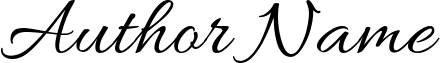
\includegraphics[width=3.6cm]{Figures/signature.png}};
\end{tikzpicture}
\end{declaration}





%----------------------------------------------------------------------------------------
%	QUOTATION PAGE
%----------------------------------------------------------------------------------------

\newpage
\thispagestyle{empty}
\vspace*{\fill}
\begin{center}
% Font family: ''Calling Angels Personal Use'' from website https://www.dafont.com

\includegraphics[width=0.8\textwidth]{Dedication/dedication.pdf}
\end{center}
\vspace*{\fill}



%----------------------------------------------------------------------------------------
%	ACKNOWLEDGEMENTS
%----------------------------------------------------------------------------------------
\begin{acknowledgements}
\setcounter{page}{2}
\addchaptertocentry{\acknowledgementname} % Add the acknowledgements to the table of contents
\vspace{1cm}


\noindent I would like to thank my mentor Tommaso Fellin for guiding me during these years. 
For his teachings and advise both in science and in life. 
For the discussions, the dedication and for always being available.
I would like to thank Stefano Panzeri and Jacopo Bonato for collaboration and helpful comments.
I would like to thank the people from Tommaso's group, a great and supportive team, for all the science and all the laughter.  
I would especially like to thank Sebastiano Curreli and Sara Romanzi, without whom this thesis would not exist. 
I would like to thank them not only for their exceptional experimental work, that produced all the data presented in this thesis, but most importantly for all the discussions, the support and for helping making the experience of doing science an exciting and enjoyable adventure. 
I would like to thank Camila for the support and the love. For \textit{todo lo todo} that she is in my life.

My highest gratitude is for my parents, Carmen and Juan. I don't have the words to thank them enough. I would like to dedicate this thesis to them.  
\\[0.4cm]

% \hfill
\begin{flushright}
    \authorname \\
    \univname \\
    \usdate\today
\end{flushright}

\end{acknowledgements}

%----------------------------------------------------------------------------------------
%	LIST OF PUBLICATIONS PAGES
%----------------------------------------------------------------------------------------
%\begin{publications}
\addcontentsline{toc}{chapter}{List of Publications}
\newcommand{\JourConfTitle}[1]{\ul{\emph{#1}}}

% ---------------------------------------------------------------------------
% JOURNALS
% ---------------------------------------------------------------------------

\begin{journals}
\item \textbf{Nan Meng}, Hayden K.-H. So, Xing Sun, and Edmund Y. Lam, ``High-dimens-ional dense residual convolutional neural network for light field reconstruction,'' \JourConfTitle{IEEE Transactions on Pattern Analysis and Machine Intelligence}, October 2019.

\item \textbf{Nan Meng}, Zhou Ge, Tianjiao Zeng, and Edmund Y. Lam, ``LightGAN: a deep generative model for light field reconstruction,'' \JourConfTitle{IEEE Access}, June 2020.

\item \textbf{Nan Meng}, Xing Sun, Hayden K.-H. So, and Edmund Y. Lam, ``Computational light field generation using deep nonparametric Bayesian learning,'' \JourConfTitle{IEEE Access}, vol. 7, pp. 24990--25000, February 2019.

\item \textbf{Nan Meng}, Edmund Y. Lam, Kevin K.-M. Tsia and Hayden K.-H. So, ``Large-scale multi-class image-based cell classification with deep learning,'' \JourConfTitle{IEEE Journal of Biomedical and Health Informatics}, vol. 23, no. 5, pp. 2091--2098, September 2019. 
\end{journals}

% \newpage
% ---------------------------------------------------------------------------
%  CONFERENCES
% ---------------------------------------------------------------------------

\begin{conferences}
\item \textbf{Nan Meng}, Xiaofei Wu, Jianzhuang Liu, and Edmund Y. Lam, ``High-order residual network for light field super-resolution,'' in \JourConfTitle{Association for the Advancement of Artificial Intelligence}, vol. 34, no.7, pp. 11757-11764, 2020.

\item \textbf{Nan Meng}, Tianjiao Zeng, and Edmund Y. Lam, ``Spatial and angular reconstruction of light field based on deep generative networks,'' in \JourConfTitle{IEEE International Conference on Image Processing}, pp. 4659–4663, September 2019.

\item \textbf{Nan Meng}, Tianjiao Zeng, and Edmund Y. Lam, ``Perceptual loss for light field reconstruction in high-dimensional convolutional neural networks,'' in \JourConfTitle{OSA Topical Meeting in Computational Optical Sensing and Imaging}, pp. CW1A.5, June 2019.

\item Edmund Y. Lam, \textbf{Nan Meng}, and Hayden K.H. So, ``Deep convolutional neural network for single-cell image analysis,'' in \JourConfTitle{High-Speed Biomedical Imaging and Spectroscopy: Toward Big Data Instrumentation and Management}, volume 10505 of Proceedings of the SPIE, pp. 105050K, January 2018.

\item \textbf{Nan Meng}, Hayden K.-H. So, and Edmund Y. Lam, ``Computational single-cell classification using deep learning on bright-field and phase images,'' in \JourConfTitle{IAPR Conference on Machine Vision Applications}, pp. 164–167, May 2017.

\item Xing Sun, Zhimin Xu, \textbf{Nan Meng}, Edmund Y. Lam, and Hayden K.-H. So, ``Data-driven light field depth estimation using deep convolutional neural networks,'' in \JourConfTitle{IEEE International Joint Conference on Neural Networks}, pp. 367–374, July 2016.

\item Xing Sun, \textbf{Nan Meng}, Zhimin Xu, Edmund Y. Lam, and Hayden K.-H. So, ``Sparse hierarchical nonparametric Bayesian learning for light field representation and denoising,'' in \JourConfTitle{IEEE International Joint Conference on Neural Networks}, pp. 3272–3279, July 2016.
\end{conferences}

\begin{patents}
\item \textbf{Nan Meng}, Xiaofei Wu, Jianzhuang Liu, ``Image Enhancement and Reconstruction based on Camera Array'', [\emph{under review}]
\end{patents}

\begin{datasets}
\item \textbf{Nan Meng}, Edmund Lam, Tsia, Kevin Kin Man, So, Hayden Kwok-Hay, ``Human somatic label-free bright-field cell images'', IEEE Dataport, 2018. [\darkred{Online}]. Available: \url{http://dx.doi.org/10.21227/H2QW97}. Accessed: Mar. 13, 2019.
\end{datasets}

\end{publications}


%----------------------------------------------------------------------------------------
%	LIST OF CONTENTS/FIGURES/TABLES PAGES
%----------------------------------------------------------------------------------------

\tableofcontents % Prints the main table of contents

\listoffigures % Prints the list of figures

%\listoftables % Prints the list of tables

\listofalgorithms % Prints the list of algorithms
\addchaptertocentry{\listalgorithmcfname}
%----------------------------------------------------------------------------------------
%	ABBREVIATIONS
%----------------------------------------------------------------------------------------
\begin{abbreviations}{ll} % Include a list of abbreviations (a table of two columns)
\textbf{mEC} & \textbf{m}edial \textbf{E}ntorhinal \textbf{C}ortex \\
\textbf{CNS} & \textbf{C}entral \textbf{N}ervous \textbf{S}ystem \\
\textbf{FOV} & \textbf{F}ield \textbf{O}f \textbf{V}iew \\
%\textbf{DLC} & \textbf{D}eep \textbf{L}ab \textbf{C}ut \\
\textbf{CNN} & \textbf{C}onvolutional \textbf{N}eural \textbf{N}etwork \\
\textbf{MSE} & \textbf{M}ean \textbf{S}quare \textbf{E}rror \\
\textbf{ROI} & \textbf{R}egion \textbf{O}f \textbf{I}nterest \\
\textbf{AP} & \textbf{A}ction \textbf{P}otential \\
\textbf{VR} & \textbf{V}irtual \textbf{R}eality \\

\end{abbreviations}


%----------------------------------------------------------------------------------------
%	SYMBOLS
%----------------------------------------------------------------------------------------
\begin{symbols}{p{0.15\textwidth}p{0.7\textwidth}l} % Include a list of Symbols (a three column table)

\multicolumn{3}{l}{\symboltitle{Global notations}}\\ \\
$I^\mathrm{SR}$ & super-resolved light field image & --- \\
$I^\mathrm{LR}$ & low-resolution light field image & --- \\
$I^\mathrm{HR}$ & high-resolution light field image & --- \\
$E^\mathrm{SR}$ & super-resolved epipolar plane image & --- \\
$E^\mathrm{HR}$ & high-resolution epipolar plane image & --- \\ \\
% $L$ & light field function & --- \\

\multicolumn{3}{l}{\symboltitle{Chapter~1}}\\ \\
$\theta$, $\phi$ & incoming direction expressed in term of spherical coordinates & rad \\
$\tau$ & time & s (second)\\
$x$,$y$ & spatial coordinates with two-plane parameterization & 1 (uint) \\
$s$,$t$ & angular coordinates with two-plane parameterization & 1 (uint) \\
$P$ & radiance distribution & \si{\watt\per\steradian \square{\metre} \text{\hertz}} \\
$\Omega$ & image plane & --- \\
$\Theta$ & parameters of the multi-layer framework & --- \\
$\gamma_s$, $\gamma_a$ & scaling factors of spatial / angular coordinates & 1 (uint) \\
$\mathcal{L}$ & loss function & --- \\ \\

\multicolumn{3}{l}{\symboltitle{Chapter~2}}\\ \\
$F_0$ & shallow features extracted by a single HConv layer & --- \\
$F_\mathrm{G_d}$ & feature maps extracted by the $d^\mathrm{th}$ HRB of the GRLNet & --- \\
$H_\mathrm{HRB}^\mathrm{n}$ & the operation of the $n^\mathrm{th}$ HRB of the SReNet & --- \\
$H_\mathrm{AGBN}$ & the operation of the proposed aperture group batch normalization algorithm & --- \\
$H_\mathrm{up}$ & upsampling operation on the low-resolution features & --- \\ \\


$\ell_A$ & angular loss & --- \\
$\ell_S$ & spatial perceptual loss & --- \\ 
$\ell_{SA}$ & the weighted combination of $\ell_A$ and $\ell_S$& --- \\
$f$ & the summation of all the feature maps after every activation function of VGG network & --- \\
$g$ & learned mapping between the low-resolution and high-resolution light field images & --- \\ \\


\multicolumn{3}{l}{\symboltitle{Chapter~3}}\\ \\
$x$,$y$ & spatial coordinates with two-plane parameterization & 1 (uint) \\
$s$,$t$ & angular coordinates with two-plane parameterization & 1 (uint) \\
$\gamma_s$, $\gamma_a$ & scaling factors of spatial / angular coordinates & 1 (uint) \\
$\ell_G$ & generator adversarial loss & --- \\
$\phi$ & denotes the mapping of VGG network & --- \\
$\delta$ & nearest neighbor downsampling operator & --- \\
$\kappa$ & a Gaussian blurring kernel with a window size of $7 \times 7$ and standard deviation of 1.2 pixels & --- \\
$\eta$ & additive noise with zero mean and unit standard deviation & --- \\ \\

\end{symbols}


%----------------------------------------------------------------------------------------
%	THESIS CONTENT - CHAPTERS
%----------------------------------------------------------------------------------------

\mainmatter % Begin numeric (1,2,3...) page numbering

\pagestyle{thesis} % Return the page headers back to the "thesis" style

% Include the chapters of the thesis as separate files from the Chapters folder
% Uncomment the lines as you write the chapters

% Chapter 1

\chapter{Introduction} % Main chapter title

\label{Chapter1} % For referencing the chapter elsewhere, use \ref{Chapter1} 

%----------------------------------------------------------------------------------------

% Define some commands to keep the formatting separated from the content 
% \newcommand{\keyword}[1]{\textbf{#1}}
% \newcommand{\tabhead}[1]{\textbf{#1}}
% \newcommand{\code}[1]{\texttt{#1}}
% \newcommand{\file}[1]{\texttt{\bfseries#1}}
% \newcommand{\option}[1]{\texttt{\itshape#1}}

%----------------------------------------------------------------------------------------

% =========================================================== %
%                 Section: Spatial navigation                 %
% =========================================================== %

\section{Spatial navigation}
\label{chap1:sec1:spatial_navigation}

The interaction between organisms and the environment is the core of life and evolution. This interaction happens at different levels with different objectives and outcomes. 
From the behavioural point of view, organisms have evolved to be able to perceive different aspects of the environment, interpret them and act in consequence. 
The more we move forward in evolution the more sophisticated and complex resources and behaviours we observe, being the nervous system, perhaps, the mayor and most interesting exponent of this. 

One of the most fundamental aspects of such interaction consists on being able to move and navigate through the environment.
A functional navigation system has to achieve a series of very difficult tasks that include the integration of information from different sensory modalities and coordination with the motor system, together with higher order cognitive processes like proprioception and goal directed activity in a flexible and dynamic way.

Spatial navigation has been extensively studied in the last 50 years, in particular, in the mammalian brain. 
The seminal work of John O'Keefe during the 1970s on rats lead to the hypothesis of a \textit{cognitive map} [REF to the book] as the way the brain solves the challenge of spatial navigation and, importantly, to experimental corroborations of the possible neuronal implementation of it. 
Unexpectedly such implementation involved the activity of specialized cells in a restricted area of the brain: \hyperref[chap1:sec:1:subsec1:hippocampus]{\textbf{The Hippocampus}}.

According to the \textit{cognitive map} theory, cells in the Hippocampus would receive inputs conveying information about sensory cues related to environmental stimuli, calculate the animal's position in space and consequently predict subsequent positions and trajectories depending on goal, inferred distances and directions. 
The ability of the internal navigation system to calculate trajectories and predict future positions represents the essence of learning in the cognitive map and has several implications regarding the internal structure, what kind of computations and types of cells should be find in the Hippocampus.

In the next sections we will summarize the anatomy and function of the Hippocampus and the different types of information encoding cells found to be present in the hippocampal navigation system.

% =========================================================== %
%                    Subsection: Hippocampus                  %
% =========================================================== %
\subsection{The Hippocampus}
\label{chap1:sec:1:subsec1:hippocampus}
Although hippocampal anatomy and connectivity has been extensively studied for decades, it's understanding and it's relationship with function is far from being completely elucidated [reference to something about discrepancies or open questions]. 
Here we will briefly described the canonical hippocampal circuit, it's constituents, structure and connectivity, paying special attention to the flow of information in the circuit.

The mammal Hippocampus is a seahorse-shaped (hence the name) brain structure located underneath the temporal lobe of the neocortex.
All mammals have a structure that could be identify as an Hippocampus, moreover, it is possible to identify a homologue of the mammalian hippocampus in all vertebrates [reference to the okeefe book, Ariens Kappers, Huber, and Crosby 1936, pp. 1248-1255, Heier 1948, Crosby, Dejong, and Schneider 1966].
It's interesting to note though, that besides the difference in structure, the Hippocampus homologues can play an entire different functional role.
The grid like structure of the Hippocampus could be thought as a general mapping structure that accomplish different functions depeneding on the species. 
In the mouse and rat, which is the case that concerns this work, is thought to be used as a spatial mapping structure, as discussed before.

In this animal the Hippocampus occupies a large portion of the forebrain and represents the paradigm of the simple cortex, consisting primarily of one basic cell type, the pyramidal or granule cells, and its asociated interneurons, the basket cells. 
In fact, a horizontal section through the posterior arch of the hippocampus shows the transition form the six layered complex structure of the entorhinal neocortex to the three layered hippocampal formation through the \textit{subiculum}.

The hippocampal structure can be divided in two U-shaped interlocking sectors, the \textit{hippocampus proper} and the \textit{dentate gyrus}. 
The hippocampus proper can, in turn, be divided in 4 subfields CA 1-4 [Lorente de No 1934]. CA stands for \textit{cornu ammonis}, another shape-like reference. 
Following the structured layer of principal neurons CA 1 appears first as the main output region of the hippocampus, followed by CA 2-3 in the regio inferior and finally CA 4 represents the scattered cells inside the hilus of the dentate gyrus. 
With the exception of CA 4, all regions of the hippocampus have a common simple structure: a compact and dense layer of cell bodies who's dendrites stretch in the same direction and receive most of their inputs from perpendicular running axons that make synapsis with many neurons at constrain regions of the dendrites. 
Such simple and preserved structure of the hippocampus represents one of the key aspects of it's function. 
The different subregions differ in the types of cells they have, CA 3 having giant pyramids, CA 1 smaller pyramids and granule cells in the dentate gyrus. 

Internally the dentate gyrus has threer layers: the \textit{granule} layer that contains the cell bodies of the mentioned granule cells, the \textit{molecular} layer consisting of the apical dendrites of the granule cells and their afferents and finally the \textit{polymorph} layer in the concave hilus of the dentate gyrus formed by the axons of the granule cells forming the mossy fiber bundle that merges with CA 4. Present in this last layer there're also some scattered basket cells interneurons.
The hippocampus proper, although it's basically a three layered structure, it can be further divided for better describing the pyramidal cells and their afferents.
First there's the \textit{alveus} layer formed by the axons of the pyramidal cells that project to the subiculum, then we find the \textit{stratum oriens} containing the basal dendrites, some basket cells and afferents from the septum.
Third, the \textit{stratum pyramidale} with the cell bodies and finally the \textit{stratum radiatum} and the \textit{stratum moleculare} with different parts of the apical dendrites.
It's interesting to note that the main feature conveying the lamination of the hippocampal structure is the nature of their afferents, briefly described next.

The connectivity in the hippocampus is highly complex and the afferents arise from many different regions of the brain, here we will describe only the canonical circuit that can be described starting with the \textbf{extrinsic afferents}. 
The main source of input to the hippocampus is the entorhinal cortex that projects from its lateral and medial regions, passing by the upper layers of the subiculum, to either the hippocampus proper through the perforant path or to the dentate gyrus through the hippocampal fisure [REF Nafstad 1967, Hjorth-Simonsen and Jeune 1972, Van Hoesen, Pandya, and Butters 1972, Hjorth-Simonsen 1973, Van Hoesen and Pandya 1975b].

Once in the hippocampus the major \textbf{interconnections between sectors} are primarily unidirectional, starting from the dentate gyrus, through CA3 and ending in CA1 [REF Lorente de No 1934, Raisman, Cowan and Powell 1965, Hjorth-Simonsen 1973, Andersen, Blackstad, and Lømo 1966, Fujita and Sakata 1962, Gloor, Vera, and Sperti 1963].   
Cells in the dentate gyrus have axons that gather together in the hilus forming the mossy fibers. The mossy fibers split in two bundles that project to the hippocampus proper. 
One bellow the pyramidal neurons in the stratum oriens, that stops abruptly in CA3.
The second bundle runs above the pyramidal cells of CA3 through the stratum lucidum and continues until the border of CA1.
CA3 and CA4 neurons make powerfull excitatory connections to the stratum radiatum of CA1 called \textit{shaffer collaterals} [REF Lorente de No 1934, Hjorth-Simonsen 1973, Andersen, Blackstad and Lømo 1966]. 
Collaterals from CA3 and CA4, potentially the same that form the \textit{shaffer collaterals}, bend and project back to the proximal dendrites of the granule cells in the dentate gyrus [REF Zimmer 1971].
It is believed that CA1 does not project back to CA3 [REF Raisman, Cowan, and Powell 1966, Hjorth-Simonsen 1973] but it is unclear if it projects to the dentate gyrus [REF Hjorth-Simonsen 1973].
Interestingly CA1 and the dentate gyrus receive inputs from CA3 of both hippocampi, including the contralateral one.
Then the information flows out of the hippocampus by CA1 cells axons that project to the septum and to the subiculum which in turn projects to back to the entorhinal cortex, closing the loop in the information flow.

Finaly, there's the \textbf{intrinsic afferents from the same sector,} that is, within each region of the hippocampus there's local connectivity in two flavours, excitatory monosynaptic connections between close by pyramidal neurons [REF Lebovitz, Dichter, and Spencer (1971)] and inhibitory polysynaptic connections due to the instrinsic pyramidal - interneuron - pyramidal loops, where the interneurons are the basket cells mentioned before [REF Kandel,Spencer, and Brinley 1961, Spencer and Kandel 1961c, Andersen, Eccles, and Løyning (1964a,b)].

To complete this brief description of the calssical hippocampal circuit we have to mention that the entorhinal cortex in turn receives a plethora of inputs from different parts of the brain, among which there are the prefrontal and cingulate cortices [REF Adey 1951, Adey and Meyer 1952, White 1959, Cragg 1965, Raisman et al. 1965, McLardy 1971, Leichnetz and Astruc 1975], the temporal cortex [REF Cragg 1965], parietal areas [Pandya and Kuypers 1969, Pandya and Vignolo 1969, Petras, 1971], pyriform cortex [REF Powell, Cowan, and Raisman 1965], the olfatory [Cragg 1960, 1961, Heimer 1968, White 1965, Price and Powell 1971, Kerr and Dennis 1972] and visual systems [REF Casey, Cuenod, and MacLean 1965, Cuenod, Casey and MacLean 1965] and the amygdala [(Krettek and Price 1974].

This is by no means a full description of the hippocampal connectivity and its afferents, but only a succinct description of the canonical pathway through which information flows in the circuit. 
In this description information flows from several regions of the neocortex and other brain region to the entorhinal cortex and subiculum, from here to the dentate gyrus, then to CA3-4, finalizing in CA1 that projects back to the subiculum and entorhinal cortex (and to the septum) closing the loop. 
Interestingly, the projections in this path are topographically precise, in the sense that, for example, a small number of cells in the dentate gyrus projects to a small number of cells in CA3.

How does such a precise and well define anatomy and connectivity structure solve the problem of spatial navigation? 
When O'Keefe first elaborated the \textit{cognitive map} theory he hypothesized that each of the three regions of the hippocampus accounted for a stage in the mapping system [REF O'keefe book].
The first stage, occurring in the dentate gyrus, would consist in organizing the environmental inputs from the entorhinal cortex and subiculum into a schema required by the mapping system. 
This complex integrations would then be transmitted to CA3-4 where the second stage of the map would take place, by representing locations in an environment and the relationship between locations.
Finally in CA1 the continuation of the map would be represented together with a mismatch system that would account for novelty or change in location information.

This very simple schematic turned out to be highly accurate in some senses and the last 4 decades of experiments have come up with empirical evidence of implementations of such system. 
The scheme has been improved and completed over the years, the current understanding in the field includes the subiculum and entorhinal cortex as part of the greater hippocampal formation.
And in each of these regions it has been found a set of highly specialized neurons that together form the spatial map. 
Many of them have been predicted in the '70 by the \textit{cognitive map} theory. 
According to it cells that encode position, distance and speed would be necessary.
In the next section we'll summarize the main types of cells of the circuit and how they fit in the overall scheme. 

% =========================================================== %
%      Subsection: Spatial information encoding cells         %
% =========================================================== %
\subsection{Spatial information encoding cells}
\label{chap1:sec:1:subsec2:spat_info_cells}
The first type of cells that conform the cognitive map were found by O’Keefe and Dostrovsky in 1971, when electrophisiological recordings in the hippocampus led to the discovery of cells that would fire predominantly in a specific location of a familiar environment.
This cells were called \textit{Place cells}. 
It's impossible to summarize here all what is currently known about place cells, so we will focus only in the main characteristics of this and the rest of the cell types of the cognitive map.

\textbf{Place cells} are mainly found in the hippocampus proper and their firing rate is modulated purely by spatial location, that is, they fire maximally when the animal's head is in a specific region of the environment. 
This region is called the \textit{place field} of the cell.  
Here we use the term environment in a generic way, but place cells have been mainly studied in constrained laboratory environments.
Interestingly, place cells have different characteristics depending on the nature of the space the animal explores.
Place cells fire at their place field location, regardless of directions of motion or speed when the animal is in a two-dimensional space, like the square/rectangular or circular boxes used in the early O'keefe experiments, but when exposed to a linear track, or one-dimensional environment, place cells would have a preferred direction of firing, and would fire much less or not at all or in a different location when the animal runs in the oposite direction [McNaughton et al., 1983; O’Keefe and Recce, 1993].
Place cells have also been found in three-dimensional environments, having three-dimensional place fields.
The latter type of place cell has been observed in bats flying through a familiar environment [Yartsev and Ulanovsky, 2013], and more recently in rodents exploring three-dimensional environments [Grieves...Jeffery 2020].

The way place cells represent position is not limited to the firing rate of the cells but also to the temporal aspect of their firing. 
Place cell firing is locked to the phase of the sinusoidal local field potential (LFP), called theta rhythm, and hence to the population activity in the hippocampus. 
The theta rhythm works as a sort of clock against which the network can measure time and temporally locate cell spikes allowing place cells to identify locations in an environment with much finer precision than if only rate codes were used.
This is called \textit{Temporal coding} [O’Keefe and Recce (1993), Huxter et al., 2003, György Buzsáki, Andreas Draguhn 2004, Buzsáki 2002].

Nearby place cells do not necessarily have nearby place fields, furthermore, a group of close by place cells would typically have place fields that span the whole space, suggesting that place cells represent a complete and highly redundant representation of the surface [O’Keefe, 1976; Wilson and McNaughton, 1994].
Once formed, these representations are stable across days [Hill, 1978; Muller et al., 1987] or even weeks [Thompson and Best, 1990].
Although, more recently, it has been suggested that not all place fields are stable [Mankin et al., 2015; Ziv et al., 2013]. 

There's a large portion of literature related to what are the necessary inputs to the hippocampus for a place cell to fire. 
This is still an unsolved question, althought there are some clear hints. 
It is clear that visual information is important, as distal cues or landmarks surrounding the environment can influence place field formation [Muller and Kubie, 1987; O’Keefe and Conway, 1978; Yoganarasimha and Knierim, 2005] but it is not necessary. 
Place cells would fire in the same location the dark in a familiar environment [Save et al., 2000; Zhang et al., 2014; Markus et al., 1994; Quirk et al., 1990], provided that other sensory cues are avialable such as olfaction or tactility. 
All this different modalities are integrated outside of the hippocampus [Jeffery, 2007], which shows that place fields are higher order representations that integrate more primitive spatial constructs such as direction, self motion and boundaries, which again talks about the inputs to the hippocampus. 
If the sensory cues show that the environment has changed or is completly new, a new and unique representation would be formed by the place cells [Anderson and Jeffery, 2003; O’Keefe and Conway, 1978] in a process called remapping [Muller and Kubie, 1987]. 
Importantly, for a map to be formed in rats and mice the animal has to explore the space directly for place cells to form a spatial representation [Rowland et al., 2011], unlike other mammals like primates that can form inferred allocentric representations of remote space if observed [Rolls, 1999; Rolls et al., 1997; Rolls and O’Mara, 1995]. 
So far we've used a rather vague definition of place cell. 
Traditionally, to define a place cell and its place field several criteria related to the firing rate, consistency of firing or reliability were used. 
Here and throughout this work we will define a place cell as a cell in the hippocampus proper that carries \textit{significant amount of information} about the animals position in it's firing activity (see methods). Later on we will define what this means in this context and how we establish significance.  

The second key cell type in the spatial representation are the \textbf{head direction cells}.  
Head direction cells are cells in the presubiculum whose firing is modulated, as the name implies, by the facing direction of the head.
They were first found by Rank [Rank 1985, 1984] and described in detailed a few years later [Taube et al., 1990a, 1990b, 1987].
Here \textit{head direction} refers to the orientation of the head in the horizontal plane.
Head direction cells are very similar in their characteristics to place cells: they have a prefer direction of firing that is independent of other behavioural factors; each head direction cell has a different preferred direction; all together, preferred directions are equally distributed in the circle, in the sense that there's no overall preferred direction of the network [Taube et al., 1990b].
Like with place cells, angular orientation of environmental cues are an important modulator of head direction cells activity [Goodridge and Taube, 1995; Taube, 1995a; Taube et al., 1990b; Zugaro et al., 2000Knierim et al., 1995] but are by no means necessary [Mizumori and Williams, 1993; Yoder et al., 2011a,b].
An interesting characteristic of this cells is that the angular relationship between preferred directions of different cells is preserved [Skaggs et al., 1995; Yoganarasimha and Knierim, 2005].
Hence when remapping an environment or if the animal is disoriented and one cell changes its orientation, the rest of the cells change theirs coherently.

With place cells and head direction cells, the cognitive map is able to build positions and to measure angles. 
The next requirement for the map to work is a way of measuring distances, to establish the metric of the map.
In 2005 a cell type that could achieve this task was found in the Moser's lab: the \textbf{grid cells}. 
Grid cells are cells that fire in multiple discrete and regularly spaced locations which form a triangular or, equivalently, an hexagonal lattice. 
This cells are found in the medial entorhinal cortex (mEC) and postrhinal cortex [Fyhn et al., 2004; Hafting et al., 2005, Fyhn et al., 2008] and in the pre- and para-subiculum [Boccara et al., 2010]. 

Grid cells have some similar characteristics to place cells or head direction cells.
Their pattern of firing arises in familiar environments and partially relies on distal visual cues, if the environmental cues rotate, grid patterns do so too consistently [Hafting et al., 2005], and deformation of the environments implies deformation of he patterns [Barry et al., 2007; Stensola et al., 2012].
Like head direction cells, the angles and distances between grid patterns of different grid cells are preserved, and when the environment rotates or moves, the patterns adapt in a coherent fashion, mantaining a stable relationship [(Fyhn et al., 2007].
This suggests that grid cells work cooperatively, as an interconected matrix known as attractor network [McNaughton et al., 2006].
Moreover, the spacing between peaks of grid patterns varies as a function of location in the entorhinal cortex. 
The scales of the patterns increase in discrete jumps as one goes from dorsal to ventral in the entorhinal cortex [Vegard Heimly Brun, et al. 2008].
Each animal can have 3 or 4 different scales. 

Finally, we have the \textbf{boundary cells}.
With yet another highly descriptive name, boundary cells, or boundary vector cells, are cells in the subiculum that respond purely to environmental boundaries.
Interestingly, the existence of boundary cells was first hypothesized after the observation that after elongating one side of a rectangular box, place fields would stretch accordingly [O’Keefe and Burgess, 1996].
This led a number of researchers to think that there could exist cells that would fire in relation to environmental boundaries, and that place cells firing could arise as a thresholded sum of a subpopulation of such cells [Barry et al., 2006; Burgess et al., 1997; Hartley et al., 2000]. 
Cells that fit such description, at least partially, were later found in several regions of the brain, like the subiculum [Barry et al., 2006], presubiculum and parasubiculum [Boccara et al., 2010], mEC [Bjerknes et al., 2014; Savelli et al., 2008; Solstad et al., 2008] and recently in the anterior claustrum [Jankowski and O’Mara, 2015] and rostral thalamus [Jankowski et al., 2015].

More formally we could define boundary vector cells as cells that fire when the animal encounters an environmental boundary in it's preferred direction.
And it's firing is driven by the memory of the boundarie's position related to the animal, based not only on perceptual cues, but also on self motion information [Lever et al., 2009; Raudies et al., 2012; Raudies and Hasselmo, 2012]. 
This definition requires that we clarify two things: first what is a boundary? A boundary can be walls, low ridges or vertical drops and the colour, texture or odour of these does not seem to influence the cell’s firing [Lever et al., 2009].
Second what does it mean to \textit{encounter} a boundary. Cells would fire at a specific disntace from the boundaries, and this distance is different for cells in different brain regions [Bjerknes et al., 2014; Solstad et al., 2008, Jankowski and O’Mara, 2015, Lever et al., 2009].

Place cells, head direction cells, grid cells and boundary vector cells lie at the core of the cognitive map and represent the most relevant more studied type of cells in the context of spatial navigation. 
However the further the cognitive map and the greater hippocampal formation is studied, the more \textit{types} of cells are found. 
Cells with more abstract or complex firing patterns, cells that respond to clear real-world correlates, but also cells that respond to more abstract or conjunctive correlates. 
We will not describe them here, but in this list we should mention \textbf{object cells}, \textbf{goal cells}, \textbf{boundary-off cells}, \textbf{perimeter cells} and \textbf{band cells}, among others. 

It's interesting to think how each of this cell types can arise, due to which inputs, and in which combinations.
In other words, what is the relation between the firing patterns of all these cell types?
Mathematically is easy to show that place cells can be formed by summing two grids of different spacing, or equivalently by summing two border cells, or that grid cells can be built by combining band cells.
The function and structure of each of this firing patterns is not yet understood.
It is however almost difficult to believe that the brain builds such an explicit and interpretable map, using specialized cells in trackable combinations.
This is of course, just the tip of the iceberg and the more the extended hippocampal formation is studied, the more cell types and complicated firing patterns appear. 

However, as intense and productive all the before-mentioned (and much more that has not been mentioned here) research has been in the last decades, we can't help but to notice that it concerns only a subgroup of the full brain network: the neurons.
But neurons represent approximately half of the cells in the brain, depending on the species can be more or less, the rest are \textbf{Glia cells}.
Although Glia cells don't have electrical activity like neurons have, they express rich calcium activity and interact with cells in active ways. 
In this work we will approach the question of if and what role play glia cells in spatial navigation in the mouse brain. 

But first we will briefly describe the types of Glia cells that can be found in the brain, focusing specially on \textbf{Astrocytes}, the main actor of this work,  their characteristics and the recent literature regarding its calcium signaling and its role in modulating neuronal activity. 

% =========================================================== %
%                      Section: Glia                          %
% =========================================================== %
\section{Glia}
\label{chap1:sec2:glia}
Glial cells have been first observed as early as the mid $19^{th}$ century by Virchow [Virchow, 1856], and better described and brought to wider attention by Santiago Ramón y Cajal and Pío del Río Hortega a few decades later thanks to the development of chloride-sublimate technique, a staining technique that targets specifically astrocytes.
At the time, glial cells were thought to play a strictly structural role in the brain.
If anything else, the terminology used to describe them would be sufficient to understand the hypothesized role: described as \textit{Zwishchenmass}, german for \textit{inbetween mass}, \textit{Nervenkitt}, or \textit{nerve glue} in english, and finally the current terminology \textit{Glial cell} comes from the Greek word \textit{gl\'ia} meaning \textit{glue}.
It wasn't until the second half of the $20^{th}$ century when electrophysiological characterization and physiological studies of glial cells permitted the understanding of the wide range of vital functions that glial cells have in the functioning of the central nervous system [Morrison and de Vellis, 1981, Bowman and Kimelberg, 1984; Kettenmann, Backus and Schachner, 1984, Cornell-Bell et al., 1990a, Araque et al., 1998; Bezzi et al., 1998]. 
Phylogenic studies show that all organisms with a central nervous system have glial cells, and, interestingly, the ratio of astrocytes-to-neurons is different depending on the animal species and on the brain region, with intriguing correlates with brain complexity and neuronal density [Herculano-Houzel, 2011, Herculano-Houzel, 2014].   
Throughout evolution, glial cells have diverge into specialized subgroups with different characteristics and function. 
The total glial population can be divided into four major groups: \textbf{microglia}, \textbf{astrocytes}, \textbf{oligodendrocytes} and their progenitors \textbf{NG2-glia}. 

Unlike the rest of the glial cells, \textbf{Microglia} originate from yolk-sac progenitors that only populate the brain during development [reviewed in Kim and de Vellis, 2005; Kettenmann et al., 2011].
They represent the main immuno-competent and phagocytic cells of the central nervous system [Filiano AJ, Gadani SP, Kipnis J August 2015], and cover the major part of adult brain in individual non-overlapping domains.
Microglia sense the environment through the movement of their filopodia, which rapidly reacts to abnormalities or damage [Nimmerjahn et al., 2005; Cronk and Kipnis, 2013].
Besides the inmuno-role, microglia has recently been hypothesized to have an active role in the healthy brain. 
Opinions on this matter are , however, controversial. 
While some studies show that microglia could be involved in motor-dependent synapse formation [Parkhurst et al. (2013)] and in features as high order as learning or social behavior [Torres et al., 2016, Kierdorf and Prinz, J Clin Invest. 2017], others have shown that ablation of microglia barely produce any alterations or pathologies in healthy adult mice [Elmore et al., 2014, 2015; Bruttger et al., 2015].
This discrepancies might be due to the major methodological differences in each study [Sarah Jäkel,and Leda Dimou 2017].

\textbf{Oligodendrocytes} are a type of large macroglia cells first observed by Pío del Río Hortega in the first half of the $20^th$ century.  
Their function is somewhat more clear: they insulate axons with self-produce myelin to allow a fast saltatory conduction and give trophic support to axons [reviewed in Nave, 2010].
However oligodendrocytes have been found in sparsely myelinated brain regions, this presumably non-myelinating oligodendrocytes might have other functions that have been so far overlooked.

More interesting are the more recently discovered oligodendrocytes precursors, the \textbf{NG2-glia} cells [ffrench-Constant and Raff, 1986].
Their first more evident function is that of forming and maintaining a homeostatic network, preserving the cell numbers stable by generating mature myelinating oligodendrocytes throughout lifetime [Dimou et al., 2008; Rivers et al., 2008; Psachoulia et al., 2009; Simon et al., 2011, Hughes et al., 2013] under physiological conditions.
What's really interesting about the NG2-glia cells is their ability to form functional synapses with neurons.
A fenomena first observed in the hippocampus [Bergles et al., 2000] but later described in other brain regions [Karadottir et al., 2005; reviewed in Sun and Dietrich, 2013].
Such synapses are uniderectional in the sense that can only receive neuronal sygnals but can't generate action potentials on their own and further propagate them [De Biase et al., 2010].

The last large group of glia cells in the brain are the \textbf{Astrocytes}.
Astrocytes and the effect of alterations on their calcium activity represent the main focus of this thesis. 
For this reason we will spend the next few sections on describing their function, anatomy and their known relation with neuronal activity. 
% \begin{figure}[!h]
%     \centering
%     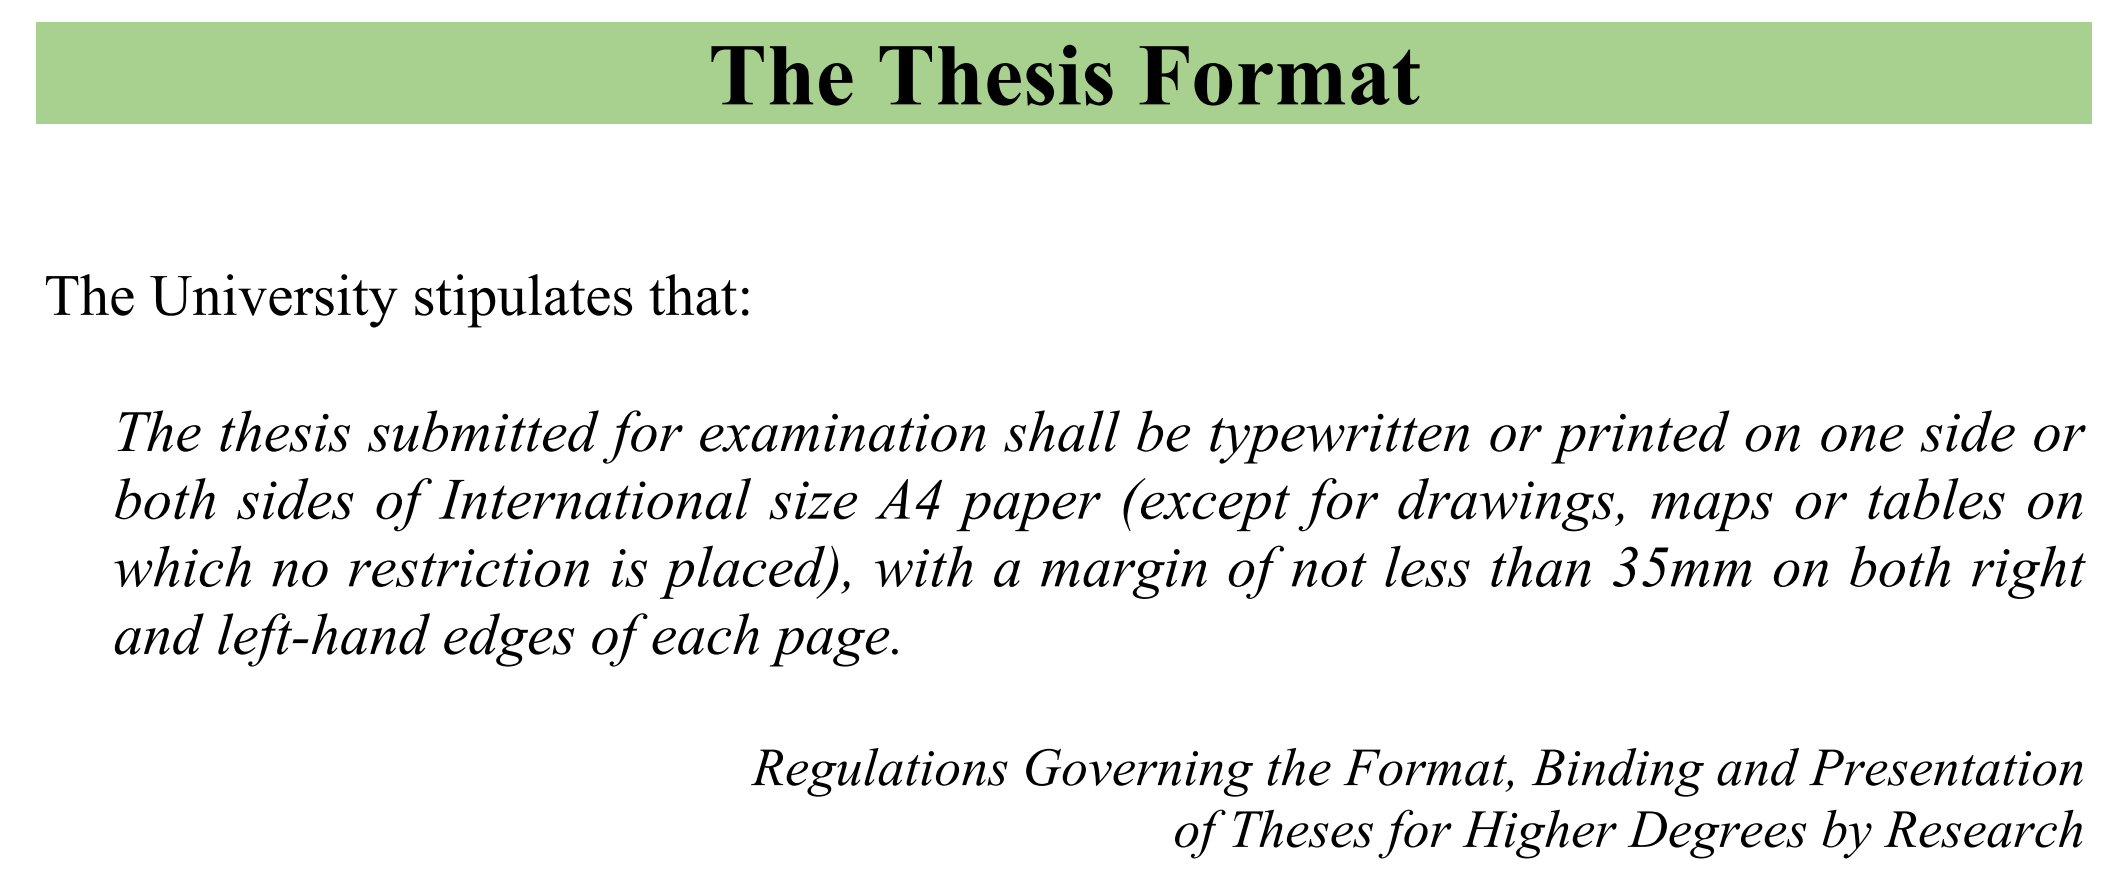
\includegraphics[width=.96\textwidth]{Figures/Chapter1/thesis_requirement.PNG}
%     \caption{Requirements of the thesis format in the Graduate School $13^\mathrm{th}$ edition booklet at Page 9.}
%     \label{fig:chap1:thesis_requirements}
% \end{figure}

% =========================================================== %
%                    Subsection: Astrocytes                   %
% =========================================================== %
\subsection{Astrocytes}
\label{chap1:sec:2:subsec1:astrocytes}
Astrocytes are the most abundant type of glial cell and represent up to $40\%$ of all the cells in the mammalian brain [Herculano-Houzel, 2014].
Despite being one of the first glial cells to be discovered around 150 years ago, their description and the understanding of their role in the brain function is far from complete.
As with everything in biology (is getting annoying really), astrocytes do not represent single homogeneous cell type and can be subdivided into several types depending on their morphology, molecular profile or function. 

From the morphological point of view astrocytes can be roughly divided into two types: \textbf{fibrous} and \textbf{protoplasmic}.
The first one is a star-shaped cell with regular contours present mainly in the white matter of the brain and spinal cord and in the optic nerve and the retina fiber layer.
Fibrous astrocytes are characterized by their elongated morphology, with long processes running parallel to the axon bundles that make contact with myelinated axons and with oligodendrocytes.
They have fewer processes compared to protoplasmic astrocytes.
Their processes spatially overlap in their domains and extend to perivascular, subpial and axonal endfeet [Lundgaard et al., 2014].

Protoplasmic astrocytes on the other hand have a “bushy” and irregular morphology, with a small round somata of $\sim 10 \mu m$ in diameter.
Present $5-10 \sim 50 \mu m$ primary processes, that further branch into thousands of branchlets and leaflets that form dense arborisations that connect with synapses [Bushong et al., 2002], and large endfeet that in turn connect with the vasculature [Nagelhus and Ottersen, 2013; Verkhratsky, Nedergaard and Hertz, 2015].
Unlike fibrous astrocytes, protoplasmic astrocytes populate mainly the gray matter in the brain and have domains with well defined borders that do not overlap between each other [Bushong et al., 2002].
Even when the the area of influence of an astrocyte is limited to local domains and do not mix with other astrocytes, it is highly connected and has a strong influence in neuronal activity.  
A single astrocyte arborisation can cover 20,000 to 80,000 $\mu m^3$, contacting 300 to 600 dendrites and potentially 100,000 individual synapses [Bushong et al., 2002, Halassa et al., 2007].
This dense connectivity allows astrocytes to control several processes like ion homeostasis or neurontransmitter recycling.
Interestingly, astrocytic domain boundaries have been proposed to be determined by, or at least closely relate to, neuronal functional units [Perea, Sur and Araque, 2014].
In this sense astrocytes could play the role of controlling and modulating \textit{functional islands} formed by the synapses confined within the area of influence of a single astrocyte [Halassa et al., 2007].
Further supports this hypothesis the fact that branching and connectivity of astrocyte, even from the same type, strongly depends on brain region.  
When comparing striatal and hippocampal astroglial populations it was noted that, despite having the same somatic volume, equivalent number of primary branches, and the same total cell volumes, hippocampal astrocyte territories are more constrained and display a tighter physical interaction with excitatory synapses [Chai et al., 2017] compare to striatal ones.

If astrocytes are so closely related to neuronal function and, as said before, have a big and dense areas of influence, what are astrocytes functions in the brain? 
This question represents still a very active area of research. Here we will enumerate some of the known functions that astrocytes fulfill but will later describe in more detail the role of astrocytes in modulating neuronal activity. 

Astrocytes are involved in the \textbf{control of cerebral blood flow} through \textbf{gliovascular coupling}.
Matching the blood flow to the neuronal metabolic needs is crucial for healthy brain functioning, this is achieved by astrocytes in a two-fold manner. 
First by regulating dilation of blood vessels: it has been proved that synaptic activity mediates cytoplasmic calcium increases in astrocytes, that in turn promote dilation of neighbouring arterioles [Zonta et al., 2003, Attwell et al., 2010].
At the same time, astrocytes regulate vasoconstriction through the release of 20-hydroxyeicosatetraenoic acid (20-HETE) [Zonta et al., 2003, Metea and Newman, 2006].
Interestingly, astrocytes seem to \textit{decide} weather to drive dilation or constriction based on local oxygen levels and metabolic states [Macvicar and Newman, 2015]. 

Given the enormous energy consumption in the brain, the regulation of oxygen and glucose availability must be tightly controlled.
This is, of course, in part regulated by blood flow. However, while oxygen freely diffuses in the brain, glucose and other metabolites need specialised transporters to travel through cell membranes.
The need for energy depends on neuronal activity, that can go from completely silent to high firing rate in miliseconds, which in turn can demand up to 30-fold increase in metabolic consumption [Attwell and Laughlin, 2001]. 
It has been demonstrated that astrocytes, who are in contact both with blood vessels and synapses, strongly and tightly control active \textbf{metabolic support} to neurons. 
This can be achieved through a variety of processes that are still an intense area of study. 
Glucose is preferentially taken by astrocytes rather than neurons [Pellerin et al., 2007], that enters glycolysis and produces lactate.
Lactate is then delivered to neurons via the astrocyte-neuron lactate shuttle (ANLS) [Pellerin and Magistretti, 1994)]. 
Meaning that astrocytes are not only involved in the metabolic support of neurons through blood flow regulation but also through direct delivery of energy substrates. 

Astrocytes, together with microglia, have a key role in the \textbf{immune response} of the brain, both in physiological and pathological conditions.
Upon brain injury or decease, astrocytes become reactive, drastically changing gene expression and entering full metal fight mode [Zamanian et al., 2012].
This changes induce morphological and functional alterations that lead astrocytes to enter one of two distinct reactivity profiles, depending on the nature of the insult. 
Inflammatory insult leads astrocytes to enter what has been called \textit{A1}, a reactivity profile implied in synapse pruning suggesting a detrimental role.
On the other hand, ischemic injury leads to activation of reactivity profile \textit{A2} responsible for growth and survival of neurons and synapses, indicating a protective role. 
Such contrasting mechanisms coexisting in the same cell type proves once more, the complexity, diversity and specificity of astrocytic function. 
Moreover, in physiological conditions, astrocytes continue to play a role in immune protection of the brain by maintaining the blood-brain barrier (BBB). 
Interestingly, astrocytes have been shown to be involved in BBB formation during development [Hayashi et al., 1997]. 

Besides the aforementioned functions, astrocytes play key roles in Ion [Sibille, Pannasch and Rouach, 2014, Nwaobi et al., 2016], water [Nielsen et al., 1997, Risher, Andrew and Kirov, 2009] and neurotransmitter [Danbolt, 2001, Herman and Jahr, 2007] homeostasis. 
Astrocytes can rapidly change their volume and intercellular communicative capacity, which allows them to redistribute water across astrocytic networks.  
Can redistribute $K^+$ ions through $K^+$ spatial buffering, and are the only cells in the central nervouse system that can synthesize glutamate and GABA from glucose. 
Astrocytes are an incredible versatile and complex cell that account for an incommensurate amount of functions and roles in the brain, however the aspect of astrocytes that concerns this work relates to the signaling in astrocytes and its relation with neuronal activity. 
We will discuss this aspects next. 
% =========================================================== %
%        Subsection: Calcium signaling in astrocytes          %
% =========================================================== %
\subsection{Calcium signaling in astrocytes}
\label{chap1:sec:2:subsec1:astro_calcium_signals}
As inexpert scientists, we PhD students have a bias view of the way research works towards positive discoveries and confirmed hypothesis. 
Simply because our biggest source of information are publications, and the chances of getting a story published that states "\textit{we formulated \textbf{this} hypothesis, and found it to be wrong}" are very low, there's a lack of charm in failure that prevents unsuccessful hypothesis to be known. 
Which is regrettable, because proven wrong hypothesis are at least as informative as positive results.
With brilliant examples like the Michelson-Morley experiment in 1887, where the two physicist trying to prove the existence of the aether, the medium in which light was thought to propagate, proved instead that it didn't exist.  
And in the way invented the interferometer. 
Invention that was later crucial for the development of the special theory of relativity and, more recently, for the detection of gravitational waves.
We can go even further and say that logic allow us \textit{only} to falsify theories, but, on the other hand, to prove a theory \textit{correct} is impossible. 
We can get encouraging results, experiments that help us gain confidence in our working hypothesis, but not really prove it.
On the other hand, one counterexample is all that is needed to prove it wrong.
As Einstein eloquently put it: \textit{The scientific theorist is not to be envied. For Nature, or more precisely experiment, is an inexorable and not very friendly judge of his work. It never says "Yes" to a theory. In the most favorable cases it says "Maybe," and in the great majority of cases simply "No." If an experiment agrees with a theory it means for the latter "Maybe," and if it does not agree it means "No." Probably every theory will someday experience its "No"—most theories, soon after conception.} [Albert Einstein: the human side: New glimpses from his archives. Dukas and Hoffman 1922]
Perhaps a way to compensate for this bias is to get rid of the miss-conception that falsifying an hypothesis represent failure but instead call it for what it is, a scientific discovery.  

In a way, a fruitful, but less interesting substitute of self-falsified hypothesis are the stories of scientist trying to prove \textit{other} peoples theories wrong, because controversy, unlike failure, sells journals.
One of the highly interesting and still active controversies in neuroscience is the question whether calcium concentration elevations in astrocytes regulates neuronal and vascular function.
This has led in the last few decades to a series of works by different groups that appeared to be contradictory, and different research lines have been seemingly proving each other wrong to give rise to a better and more profound understanding of the subject.  
We will not refer here the complete story that has been brilliantly summarized by Bazargani and Attwell [Bazargani and Attwell 2016], but will refer only some characteristics of calcium signaling in astrocytes that are relevant for the understanding of this work.

It's important to note first, that astrocytes, unlike neurons, are non-excitable cells.
For this reason, $Ca^{2+}$ fluctuations have been considered as the main intracellular readout of detection of environmental changes.
That includes astrocyte-neuron communication. 
An extensive amount of work in the last few decades has been dedicated to understand the origin of $Ca^{2+}$ transients, if this fluctuations are somehow relevant for neuronal regulation, and if so, how.
To the date most of this questions remain unanswered, although currently there seems to be a common consensus in the field that (spoiler alert) they are at least involved in several regulation pathways, and respond, in physiological conditions to behavioral and sensory correlates. 

Should caught our attention the fact that baseline levels of $Ca^{2+}$ in astrocytes are higher than that of neurons, and that this concentration vary inside each cell, being higher in processes compared to the soma [Zheng et al., 2015].
Which already suggest two observations: first, the relevance of $Ca^{2+}$ in astrocytic signaling, and second, the within-cell complexity of it. 
In astrocytes, $Ca^{2+}$ fluctuations can have different sources, the first of which is intrinsic. 
In fact, it was shown that $65\%$ of astrocytes in hippocampal slices exhibit asynchronous and localised $Ca^{2+}$ transients, even in the absence of neuronal activity [Nett et al., 2002].
The role and relevance of these untriggered events has yet to be defined. 
Specially because it's unclear if this spontaneous events do happen in physiological conditions and if so, in which fashion. 

More interesting are \textbf{$Ca^{2+}$ changes induced by neuronal activity}.
Glutamate has been shown to evoke calcium concentration rise in astrocytes in several contexts, in culture [Cornell-Bell et al., 1990], in brain slices [J.W. Dani et al., 1992], in whole retina [Newman and Zahs 1997] and \textit{in vivo} [Wang et al. 2006].
This calcium transients can propagate along astrocyte processes and even between glial cells [ornell-Bell et al., 1990, J.W. Dani et al., 1992, Hirase, H. et al., 2004, Nimmerjahn, A. et al., 2004].
This observations further support the possibility that glial Ca2+ waves might constitute an extra-neuronal signaling system in the CNS, and, importantly, that it can be driven by neuronal activity. 
However, to begin to understand the neuron-astrocytic $Ca^{2+}$ activity relation one must realize that, just like neurons, astrocytes have to be thought as the sum of many different subcellular compartments and that calcium transients occurring in the soma are very different and can have different sources as the the ones in fine astrocytic processes near synapses.
$Ca^{2+}$ events in processes can occur independently of larger ones in the soma, which suggest that regulation of synapses or blood vessels can happen locally. 
This events can, however, propagate to neighbouring intracellular areas [Di Castro et al., 2011] or even synchronise with neighbouring cells [Takata et al., 2013].
Importantly, it has been shown that such events correlate with the strength of neuronal activity [Panatier et al., 2011].

Process and soma $Ca^{2+}$ events also differ in their temporal profile.
While is true that somatic calcium transients are several order of magnitude longer than neuronal action potentials, which has been an historical argument against the hypothesis that astrocyte could be involved in real-time information processing in the brain, smaller events occur in processes even in the subsecond scale [Winship, Plaa and Murphy, 2007; Lind et al., 2013, 2018].
This partially solves the temporal argument, but in a more fundamental aspect, it's by no means clear if information processing in neuronal network relies in temporal or rate coding or a combination of both.
Rate coding responses could be an alternative way in which long lasting astrocytic $Ca^{2+}$ signals could be involved in a relevant temporal scale in neuronal activity and information processing [Semyanov, 2019].
On a further bigger scale, $Ca^{2+}$ events can propagate as waves through networks of several tens and even hundreds of astrocytes.
Behavior that  has been observed in cultures [Cornell-Bell et al., 1990b], as well as \textit{in vivo} in the frontal and parietal cortices upon sensory stimulation []Ding et al., 2013] and in the cerebellum during locomotion [Nimmerjahn, Mukamel and Schnitzer, 2009].
Giving rise to the possibility of astrocytes modulating neuronal activity at a network scale. 

As stated before, many of such calcium transients have been shown to depend, or have its origin in neuronal activity dependent processes. 
In hippocampal dentate gyrus astrocytes action potential–driven synaptic transmitter release triggers large and long lasting ($\sim3 s$), spatially broad ($\sim12 \mu m$) events, while spontaneous synaptic transmitter release produces brief ($\sim 0.7 s$), spatially localized ($\sim 4 \mu m$) transients [Di Castro, M.A. 2011].
It has been suggested that release of $Ca^{2+}$ from internal stores could be the main source of $Ca^{2+}$ somatic transients, while in the astrocyte processes transmembrane entry of Ca2+, presumably through endogenously active channels such as TRPA1 [Shigetomi, 2012] or receptor-gated $Ca^{2+}$-permeable ion channels, generates 30–40\% of $Ca^{2+}$ concentration elevations. 
In this way while $Ca^{2+}$ rises in astrocyte somata may be too slow [Schummers, et al. 2008, Schulz, K. et al, 2012] to generate rapid blood flow increases, $Ca^{2+}$ transients in the processes that are faster than in the soma [Tang, W. et al. 2015] occur before or with a similar time course to the increase of blood flow [Lind, B.L. 2013, Otsu, Y. et al, 2015].

We will not dig into the specific mechanisms through which neuronal activity could induce such calcium transients (related to the activation of mGluR receptors by glutamate release) or the controversies involved. 
But will instead mention some of the observations that evidence astroctytic calcium transients physiological relevance. 
It has been observed that whisker stimulation increases $Ca^{2+}$ concentration in astrocytic cytoplasm in the barrel cortex [Wang et al., 2006], in a frequency dependent manner [Perea and Araque, 2005; Sherwood et al., 2017]. Other behavioural variables like locomotion or arousal state have been observed to evoke $Ca^{2+}$ elevation over broad spatial areas, mediated by noradrenaline signals in the frontal and parietal cortex [Ding et al., 2013, Paukert, et al., 2014].
Suggesting an astrocytic involvement in the control and modulation of sensory input and behavior. 
% =========================================================== %
%   Subsection: Astrocityc modulation of neuronal activity    %
% =========================================================== %
\subsection{Astrocityc modulation of neuronal activity}
\label{chap1:sec:2:subsec2:astro_neuromodulation}
The complexity both in source and dynamical properties of calcium oscillations in astrocytes makes it rather complicated but at the same time extremely interesting to study.
We've seen that astrocyte calcium changes are related to neuronal activity, to neurotransmitter release and to sensory input and behavioral state.
That they can occur in fast transients in the processes or in longer, stronger events in the soma. 
That can propagate within the cell, across neighbouring cells and through extended networks.
This covers one way of information flow in the \textit{extended brain network} (that is considering neurons and glial cells). 
But what is the role (or roles), if any, of each of this astrocytic calcium dynamics in the processing of information by neuronal networks?
In other words, how does astrocytic activity modulate neuronal functioning?
We are interested in the answers to this questions that are related to the brain information processing and its meaning for behavioural outputs, and therefore to the astrocytic-induced changes in neuronal properties. 

Given that astrocytes extend processes that are ideally positioned for dynamic exchange with the synapses, the first observations are related to how astrocytes influences synapses, this happens in three aspects: by regulating \textbf{presynaptic release probability}, \textbf{postsynaptic receptor activation} and \textbf{synaptic plasticity}.
Importantly, release of gliotransmitters, which is one of the key ways in which astrocytes comunicate with neurons, is widely accepted to follow cytoplasmic $Ca^{2+}$ rise in astrocytes, making $Ca^{2+}$ transients highly relevant for the comunication between neurons and astrocytes and its experimental testing.
However, we have to keep in mind that gliotransmitters can have different effects depending on the target, the neuronal activity regime, the brain region, and the developmental state to be able to properly interpret the extended network activity. 

At the \textbf{presynaptic level}, it has been observed that in the dentate gyrus, astroglial glutamate release activates presynaptic NMDA receptors, potentiating excitatory transmission [Jourdain et al., 2007].
Similarly, in the hippocampus proper glutamate potentiate transmitter release, although in this case by activating presynaptic mGluRs but without the intervention of NMDA receptos [Perea and Araque, 2007; Navarrete and Araque, 2010].
Astrocyte release of glutamate has been observed to mediate not only excitation but also inhibition at the presynaptic level during sustained neuronal activity.
This is achieved in two ways, first by binding presynaptic kainate receptors that strengthen inhibitory synaptic transmission [Kang et al., 1998; Liu et al., 2004], and second, $Ca^{2+}$ uncaging-mediated glutamate release from astrocytes produce binding of presynaptic mGluRs in neurons that in turn decrease evoked postsynaptic currents in the hippocampus [Araque et al., 1998].
It has been recently shown that single astrocyte may release different gliotransmitters [Covelo and Araque, 2018], which can induce more complex modulation of synapses: high frequency stimulation of the CA3-CA1 projection in the hippocampus produced finely tuned release of both glutamate and adenosine from astrocytes, modulating synapses in a biphasic way.
Initial glutamate release induced potentiation followed by purinergic-mediated depression of neurotransmitter release, which represents an elegant example of the subtle and complex modulation effects of neuronal comunication by astrocytes. 

At the \textbf{postsynaptic level} it has been observed that disrupting gliotransmission in a dnSNARE mouse model produced a hypofunction of postsynaptic NMDA receptors, which has effects at the network level affecting cortical slow oscilations (see bellow) [Fellin et al., 2009].
Similarly NMDA receptors binding have been shown to be modulated by astroglial D-serine release, which in turn modulates glutamatergic synaptic transmission [Panatier et al., 2006, Henneberger et al., 2010].

Astrocyte gliotransmission has been observed to have effects in \textbf{synaptic plasticity} and memory.
Clamping $Ca^{2+}$ in individual CA1 astrocytes blocks LTP inductions at nearby excitatory synapses by decreasing the occupancy of the NMDAR co-agonist sites [Henneberger et al., 2010].
Exogenous D-serine or glycine application reverse this effect.
Note that this $Ca^{2+}$-dependent release of D-serine from an astrocyte control of NMDAR-dependent plasticity can potentially affect many thousands of excitatory synapses but only those that are nearby, implying a local regulation of neuronal activity. 
This further advocates for the functional spatially localized aspect of astrocytic domains.   
Conversely, astrocytes can also modulate synaptic depression. 
$Ca^{2+}$ clamping in rat barrel cortex astrocytes during development showed impaired t-LTD [Min and Nevian, 2012].
Moreover, simultaneously stimulating an astrocyte with depolarising pulses and afferent fibres resulted in LTD.
This result suggests that astrocyte signalling is sufficient to induce plasticity at the level of neuronal synapses. 
Finally, astrocytes have been shown to be involved in the synaptic depression of untetanised synapses paralleling LTP in the hippocampus [Pascual et al., 2005; Serrano et al., 2006; Andersson, Blomstrand and Hanse, 2007; Chen et al., 2013]

There are several mechanisms through which astrocytes modulate \textbf{neuronal excitability}, that is, neuronal electrical dynamics during action potential firing. 
Action potentials or spikes in neurons depend on the fine and complex relation between ionic concentrations withing neurons and in the extracellular space, which is in turn regualted by the activity of voltage-gated ion channels.
One of the most consolidated functions of astrocytes is the maintenance of ionic homeostasis and more specifically the buffering of extracellular potassium [Kofuji and Newman, 2004, 2010; Kimelberg and Nedergaard, 2010; Hertz and Chen, 2016].
The rapid intake of $K^+$ by astrocytes prevents neuronal hyperexcitability [Bellot-Saez et al., 2017]. 
Although the specific intracellular mechanisms are not clear, there has been strong evidence towards the idea that astrocytes, through the secretation of purines set neuronal firing thresholds, both in pyramidal cells and interneurons [Kawamura, Ruskin and Masino, 2010, Kawamura et al., 2004, Tan et al., 2017].

We mentioned how astrocytes modulate each side of the synapse and synaptic plasticity and later how they influence neuronal excitability, continuing with the growing scale progression astrocytes play key roles in the \textbf{synchronization of neurons} and at the \textbf{network level}.
As we stated at the beginning of this section, the mechanisms through which astrocytes influence neuronal activity depend on cell type, brain region and developmental state of the animal.
In the absense of neuronal activity hippocampal CA1 neurons present inward currents with slow kinetics found to be mediated by glutamate released from astrocytes, simillar to those observed under stimulation of Schaffer collaterals [Fellin et al., 2004].
This response occurs synchronously in multiple CA1 neurons, evidencing the functional role of astrocytes in the synchronization of neurons.
More recently, it has been observed that cellular coordination might not involve inter-astroglial Ca2+ spread, suggesting other mechanisms of astroglial networks cell coordination [Chever et al., 2016]. 
However, neuronal network oscilations or brain waves are not restricted to the hyppocampus, instead they are present in almost every brain region, during sleep, sensory perception, can have functions that vary from memory consolidation to temporal coding (as mentioned before) and lie in a wide variety of frequency and power bands.   
The mechanisms by which network oscillations are formed and modulated are still a matter of intense study.
Interestingly, it has been recently proposed that astrocytes might play a role in the regulation of neuronal membrane potential oscillations at a wide range of frequencies [Bellot-Saez et al., 2018].
Indeed blockade of $K^+$ uptake or astrocytic connectivity, enhance network excitability and form high power network oscillations.
This could be due to changes in the oscillatory behaviour of individual neurons, which is a well known effect in the system dynamics field.
More precisely it has been shown that, as we mentioned before, impairing gliotransmission altered slow wave dynamics in the cortex by reducing neuronal depolarization periods duration, and prolonging hyperpolarization [Fellin et al., 2009].
Moreover, slow oscillations involves oscilation in neuronal membrane potential as well as astrocytic calcium dynamics, with the latter preceding neuronal changes.   
resulted in altered cortical slow oscillations through a reduction in the duration of neuronal depolarisation, and prolonged hyperpolarisation (Fellin et al., 2009). In agreement with this report, simultaneously monitoring Ca2+ activity in neurons and astrocytes during slow wave activity revealed that both types of cells are recruited during slow wave oscillations in vivo, with the astroglial Ca2+ synchronisation arising before the neuronal one. 
And alterations in astrocytic calcium dynamics inhibits slow wave activity, showing the fine causal interplay between both types of cells during brain oscillations [Szabó et al., 2017].
Finally, astrocytic signaling has been observed to be involved not only in gamma oscillations but also in their cognitive correlates [Lee et al., 2014], being this an example of how astrocytes acitivity is crucial for proper performance in tasks as high order as novel objet recognition.

We couln't and wouln't try to make a full description of the vast plethora of mechanisms by which neurons and astrocytes interact, or the function of each of this interactions, many of which are a matter of active debate to date. 
Heterogeneity in experimental procedures might account for some of the discrepancies in the literature.
But we hope we've built so far the case that astrocytes, and in particular astrocytic $Ca^{2+}$ dynamics, is involved and regulates the way the brain process information.
It does so at the level of the synapses, in single cells, and at the network scale.
That this interactions go both ways, with astrocytes modulating neuronal dynamics but also neuronal 
activity interfering in astrocytic profiles.
That the complexity and richness of this modulation extendes not only to the spatial domain but also at the temporal scale, with small fast and local interactions as well as large waves of activity spaning whole brain regions.
And more important that when studying the way the brain solves a task, considering only neuronal networks might not be enough, and a shift in the paradigm towards the study of an extended neuronal-glial networks might be needed. 

% =========================================================== %
%        Subsection: Astrocytes accumulate evidence           %
% =========================================================== %
\subsection{Astrocytes accumulate evidence}
\label{chap1:sec:2:subsec4:astro_evidence}
So far we have been dealing with how astrocytes can be involve the way in which neurons process information, but a parallel and relevant question is if and how astrocytes process information themselves. 

Refer to paper from \textit{Misha Harens}


% ================================================================ %
% Section: Astrocytes encode spatial information in Ca2+ activity  %
% ================================================================ %
\section{Astrocytes encode spatial information in $Ca^{2+}$ activity}
\label{chap1:sec3:astro_spat_info}

% =========================================================== %
%        Subsection: Astrocytes and information               %
% =========================================================== %
\subsection{Astrocytes and information}
\label{chap1:sec:3:subsec1:astro_info}
Treating astrocytes $Ca^{2+}$ activity with Information theory approaches

% =========================================================== %
%             Subsection: Decoding of position                %
% =========================================================== %
\subsection{Decoding of position}
\label{chap1:sec:3:subsec2:position_decoding}

% =========================================================== %
%                    Subsection: Page Margin                  %
% =========================================================== %
% \subsection{Page Margin}
% \label{chap1:sec:2:subsec1:page_margin}
% The format of page size and margin is defined in ``main.tex'' file \textbf{Line 63-71}. The page margin of the current version template is \uline{Left: 35mm, Right: 36mm (a4paper).} Users can change the page margin by adjusting the corresponding settings. There is no stipulation for the top and bottom margins, but the booklet recommend that both of them should be 25mm, which is adopted in this template. 


% =========================================================== %
%          Subsection: Font, Alignment, Line Spacing          %
% =========================================================== %
% \subsection{Font, Alignment, Line Spacing}
% Ordinarily, there is no restrict stipulation for the font family, font size, alignment, and line spacing. All of these are a matter of personal preference. This template uses \textit{10pt} font size, \textit{Fully Justified} alignment style and \textit{One and A Half} line spacing. Users can adjust the settings in \textbf{Line 19-33} of the ``main.tex'' file to change the typeset.


% =========================================================== %
%                      Subsection: Contents                   %
% =========================================================== %
% \subsection{Contents}
% The contents of this template can be subdivided into three parts --- the front matter, the text and the back matter, which strictly follows the stipulations of the official booklet (Page 17). \tabref{chap1:longtable:checking_list} indicates the what contents are required in the submitted thesis and what contents are optional. The column ``Required'' denotes that 
% \begin{center}
% \begin{longtable}{|l|c|c|}
% \caption{Checking list indicating the contents should be included in the thesis.}\label{chap1:longtable:checking_list}\\
% \hline
% \textbf{The Front Matter} & Required     &  Include $\checkmark$ \\ \hline \hline
% Abstract                  & Yes          & $\checkmark$         \\
% Title Page                & Yes          & $\checkmark$         \\
% Frontispiece              &              &                      \\
% Dedication                &              & $\checkmark$         \\
% Epigraph                  &              &                      \\
% Declarations              & Yes          & $\checkmark$         \\
% Acknowledgements          &              & $\checkmark$         \\
% Table of Contents         & Yes          & $\checkmark$         \\
% List of Illustrations     &              &                      \\
% List of Figures           &              & $\checkmark$         \\
% List of Tables            &              & $\checkmark$         \\
% List of Algorithm         &              & $\checkmark$         \\
% List of Abbreviations     &              & $\checkmark$         \\
% List of Symbols           &              & $\checkmark$         \\
% Others                    &              &                      \\ \hline \hline
% \textbf{The Text}         & Yes          & $\checkmark$         \\ \hline \hline
% \textbf{The Reference or Back Matter} &    ---    &   ---       \\ \hline \hline
% Glossary                  &              &                      \\
% Appendices                &              &                      \\
% Notes                     &              &                      \\
% Bibliography or Reference List & Yes          &  $\checkmark$   \\
% Index                     &              &                      \\
% \hline
% \end{longtable}
% \end{center}
% This template support most of the contents listed in the figure, including the ``Abstract'', ``Title Page'', ``Declarations'', ``Acknowledgements'', ``List of Publications'', ``Contents'', ``List of Figures'', ``List of Tables'', ``List of Algorithms'', ``List of Abbreviations'', ``List of Symbols'', ``Main Text'', ``Appendices'', and ``Bibliography''. Each part is defined in an independent tex file and the ``main.tex'' file combines all the different parts to form the entire thesis. Therefore, users can easily make the changes by adjusting the corresponding document files.

% In addition to the stipulations of the booklet, this template also provides a beautiful \textbf{cover page}, which is the first two pages of this project. \uline{The cover page is \textbf{not required} by the Graduate School and you'd better remove the cover page when bounding your thesis for submission.}









% Chapter 2

\chapter{Rational and Aim} % Main chapter title

\label{Chapter2} % For referencing the chapter elsewhere, use \ref{Chapter2} 

%----------------------------------------------------------------------------------------

% Define some commands to keep the formatting separated from the content 
% \newcommand{\keyword}[1]{\textbf{#1}}

%----------------------------------------------------------------------------------------

% Maximum one page, just to state the logical flow in a few sentences and what we gonna do.
% We know that:
% \begin{itemize}
%     \item Astrocytes encode spatial info in Ca2+ activity
%     \item Ca2+ in astrocytes modulates neuronal activity
% \end{itemize}
% That brings us to the questions:
% \begin{itemize}
%     \item What is the functional role of the Ca2+ signaling in astrocytes in spatial information encoding?
%     \item Does modulation of Ca2+ in astrocytes alter spatial encoding in neurons? how? 
% \end{itemize}
% To address this questions we used 1p and 2p imaging + cell specific chemogenetic manipulation in the mouse hippocampus.

% \textbf{You also need to write the rationale and aim page. This is done as follows: 
% first you state a few sentences about the scientific background of the project (starting from spatial navigation and ending to astrocyte calcium dynamics) and you build the case; 
% then you state your hypothesis (astrocyte calcium dynamics modulate neuronal spatial representation; 
% you mention what you did, how you did it, and what you found; 
% you end with a sentence that summarizes the impact of your work on current knowledge. 
% (all of this can be done taking what is already written in the intro and results).}

Neural place cells in the hippocampus encode navigational information through the modulation of their firing rate as a function of the animal’s spatial location [\cite{okeefe1976}], providing a cellular substrate for spatial cognition. 
Whether navigational information is processed exclusively in neuronal cells or it involves other cell types in the brain is currently unknown. 
Astrocytes, a major class of glial cells in the brain, display complex dynamics in their intracellular calcium concentration [\cite{bazargani2016}]. 
These intracellular signals can be spatially restricted to individual subcellular domains (e.g., cellular processes vs somas), be coordinated across astrocytic cells, and trigger the release of neuroactive molecules which deeply influence synaptic transmission and neuronal excitability.
Recent unpublished work from my mentor’s laboratory in collaboration with Jacopo Bonato and Stefano Panzeri shows that astrocytes encode navigational information in their intracellular calcium dynamics, suggesting that astrocytes may contribute to the modulation of the neuronal representation of space. 
In this thesis work, I developed an analysis pipeline to directly test this hypothesis using statistical methods and Information Theory approaches. 
The developed analytical tools were applied to two experimental data sets in which neuronal place cells in the hippocampus were imaged using two-photon microscopy while selectively manipulating astrocytic calcium dynamics with pharmacogenetics during virtual navigation. 

% This chapter demonstrates how to make changes and DIY the thesis style when using this template. For each component of the thesis, we provide both 

% \section{Title Page}
% \textbf{Title Page} is designed to obviously bear the title of the thesis and the author's name. Users can add any degrees or professional qualifications that he/she holds as well as the author's name in the national script. Both the title and the author's name are highlighted in blod style. Given that there may also be an oral and/or written examination, and thus this template uses the following form of words:

% \begin{quote}
% A thesis submitted in partial fulfilment of the requirements for the degree of Doctor (or Master) of Philosophy at The University of Hong Kong.
% \end{quote}

% \noindent The title page is not numbered, or counted in the pagination of the front mater, or listed in the table of contents. The document for title page is quite simple, which can be found in the path \colorbox{gray!20}{Titlepage/titlepage.tex}.


% \section{Dedication}
% \label{chap2:sec2:dedication}
% \textbf{Dedication} is a place to show your wish to dedicate the thesis to friends, family or loved ones. This template uses a single page example for dedication, as shown in \figref{fig:chap2:dedication_sample}. This page is not numbered, or counted in the pagination of the front matter, or listed in the table of contents.
% \begin{figure}
%     \centering
%     
\includegraphics[width=.6\textwidth]{Dedication/dedication.pdf}
%     \caption{An example dedication page.}
%     \label{fig:chap2:dedication_sample}
% \end{figure}


% \section{Epigraph}
% \label{chap2:sec3:epigraph}
% \textbf{Epigraph} is a relevant quotation on the subject of the thesis, or some general guidelines or philosophical principles. Ordinarily, the author and source of the quotation should also be given. This page is not included in the template and users can add the epigraph page according to their willingness.


% \section{Declarations}
% \label{chap2:sec4:declarations}
% \textbf{Declarations} page is a required item according to the official booklet. The contents of declaration are in terms of the official sample (\textit{Sample Page 6} on page 41 of the booklet) with some minor changes to specify the author's name and thesis title.


% \section{Acknowledgements}
% \label{chap2:sec5:acknowledgements}
% \textbf{Acknowledgements} is the place where the author thanks mentors, labmates, colleagues, friends, family members and also the financial support from scholarships and research grants. Each page of the acknowledgements is numbered in lower case Roman numerals


% \section{Table of Contents}
% \label{chap2:sec6:table_of_contents}
% \textbf{Table of Contents} in this template is simply headed ``Contents'' which lists all the parts of the thesis and the page on which they commence. Each of the chapters, sections and subsections are included in the list. The capitalization and wording of the titles listed in the table exactly agree with the corresponding ones appear in the body text. If users would like to include some optional pages in the Table of Contents, such as the Frontispiece page or Epigraph page, they can simply add a command \verb|\addchaptertocentry{\pagename}| at the corresponding page. For example, your can add the \textit{Abstract} item to the Table of Contents, by adding the command to the file \codestyle{Abstract/abstract.tex}, as shown in \figref{fig:chap2:example_add_command}.
% \begin{figure}[!h]
%     \centering
%     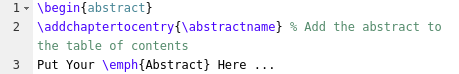
\includegraphics[width=.8\textwidth]{Figures/Chapter2/add_command_example.png}
%     \caption{An example of how to add chapter to the Table of Contents.}\label{fig:chap2:example_add_command}
% \end{figure}


% \section{List of Tables, Figures and Algorithms, etc}
% \label{chap2:sec7:list_of_tables_figures_and_algorithms_etc}
% \begin{figure}[t]
%     \centering
%     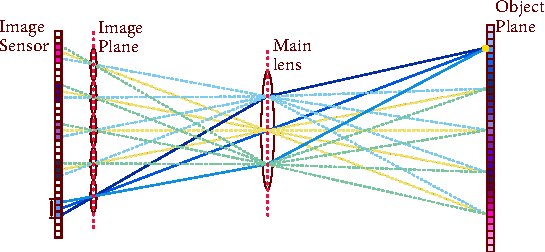
\includegraphics[width=0.6\textwidth]{Figures/Chapter2/photo_consistency.pdf}
%     \caption{Light transformation model in a plenoptic camera. Within a plenoptic camera, a micro-lens array has been placed at the image plane, which further splits the incoming light rays from different directions and records them separately. Therefore, the multi-view information can be extracted from each light field image captured by a single shot.}
%     \label{fig:photo_consistency}
% \end{figure}

% \begin{figure}[t]
%     \centering
%     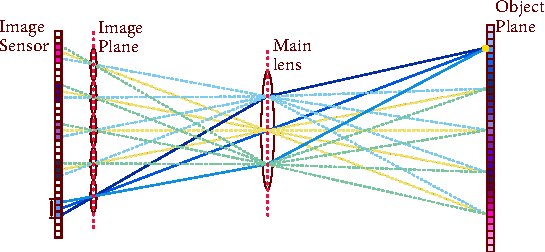
\includegraphics[width=0.6\textwidth]{Figures/Chapter2/photo_consistency.pdf}
%     \caption[Light transformation model (focused on the plane).]{Light transformation model in a plenoptic camera. Within a plenoptic camera, a micro-lens array has been placed at the image plane, which further splits the incoming light rays from different directions and records them separately. Therefore, the multi-view information can be extracted from each light field image captured by a single shot.}
%     \label{fig:photo_consistency_with_nickname}
% \end{figure}
% Following the Table of Contents, the template includes the lists of tables, figures and algorithms, abbreviations and symbols. The numbering, capitalisation and wording of the titles of every items listed agree exactly with the manner in which they appear in the body text. For the illustration with a long title, users can also provide a ``nickname'' of the illustration by enclosing the it in the square brackets. For example, \figref{fig:photo_consistency} and \figref{fig:photo_consistency_with_nickname} have the same image captions in the body text, but the wordings appear in the Table of Contents are different. \figref{fig:photo_consistency_with_nickname} uses the wordings in the square brackets as its caption, as shown at page \darkred{vii}.

% Chapter 3

\chapter{Materials and Methods} % Main chapter title

\label{Chapter3} % For referencing the chapter elsewhere, use \ref{Chapter3} 

% =========================================================== %
%          Subsection: Experimental procedures                %
% =========================================================== %
\section{Experimental procedures}
\label{chap3:sec:1:exp_proc}
\subsection{Animals}
All experiments involving animals were approved by the National Council on Animal Care of the Italian Ministry of Health and carried out in accordance with the guidelines established by the European Communities Council Directive authorization (61/2019-PR). 
From postnatal days 30, animals were separated from the original cage and group housed (2–5 per cage) in a 12-hours light-dark cycle with \textit{ad libitum} access to food and water. 
Only animals older than 10 weeks underwent experimental procedures. 

\subsection{AAV injection and surgery for chronic hippocampal imaging}
\label{chap3:sec:1:subsec2:AAV_injection}
Neuronal-specific GCaMP6f expression was obtained using AAV1.CamKII.GCaMP6f.WPRE.SV40 (Addgene viral prep \# 100834-AAV1).
Astrocytic-specific GCaMP6f expression was obtained using pZac2.1 gfaABC1D-cyto-GCaMP6f (Addgene viral prep \# 52925-AAV5 a gift from Dr. Khakh, \cite{haustein2014conditions}; \cite{srinivasan2015}).
Astrocytic-specific DREADD expression was obtained using AAV-GFAP-hM3D(Gq)-mCherry (Addgene viral prep \# 50478-AAV5)

Male C57Bl6/j mice were placed into a stereotaxic apparatus (Stoelting Co, Wood Dale, IL), maintained on a warm platform at $37^{\circ}$C and anesthetized with 2\% isoflurane/0.8\% oxygen. 
Before surgery, a bolus of Dexamethasone (4 mg/kg, Dexadreson, MSD Animal Health, Milan, IT) was provided with an intramuscular injection. 
A small circular craniotomy (diameter, 0.5 mm) was drilled on the right hemisphere (1.75 mm posterior, 1.35 mm lateral to bregma) after scalp incision. 
A micropipette loaded with AAV was then lowered into the CA1 region of the hippocampus (1.40 mm deep to bregma). 
800 nl of solution containing the two AAVs for GCaMP6f (dilution, 1:5) and DREADD (dilution, 1:8) was injected at 100 nL/min using a hydraulic injection apparatus driven by a syringe pump (UltraMicroPump, WPI, Sarasota, FL). 
After viral injection, a stainless-steel screw was positioned on the skull of the left hemisphere and a chronic hippocampal window was implanted following (\cite{dombeck2010}, \cite{sheffield2015}). 
A 3 mm craniotomy centered at coordinates 2.00 mm posterior and 1.80 mm lateral to bregma was opened using a drill and the dura was removed using fine forceps. 
A blunt needle coupled to a vacuum pump was used to carefully aspirate the cortical tissue overlaying the hippocampus. 
The exposed tissue was continuously irrigated during aspiration with HEPES-buffered artificial cerebrospinal fluid (ACSF). 
Aspiration was interrupted when the thin fibers of the external capsule were visible. 
A cylindrical cannula-based optical window was then positioned at the craniotomy touching the external capsule. 
A thin layer of silicone elastomer (Kwik-Sil, World Precision Instruments, Sarasota, FL) was used to fill and isolate the space between the steel surface of the optical window and the brain tissue. 
Epoxy glue was used to attach a custom stainless-steel headplate to the skull.
Black dental cement was used to secure each component in place.
An intraperitoneal bolus of antibiotic (BAYTRIL, Bayer, DE) was administrated to animals after surgery.

Optical windows consisted of stainless-steel cannula segments with thin walls (outer diameter, 3 mm; inner diameter, 2.77 mm; height, 1.50 - 1.60 mm). 
At one end of the cannula a 3.00 mm diameter round coverslip was attached by means of UV curable optical epoxy (Norland optical adhesive 63, Norland, Cranbury, NJ). 
Bonding residues and Edges were smoothed with a diamond coated cutter.

\subsection{Two-photon imaging}
Two-photon calcium imaging was performed using an Ultima Investigator or an Ultima II scanheads (Bruker Corporation, Milan, IT) equipped with raster scanning galvanometers (mirror dimension, 6 mm or 3 mm) a 16x/0.8 NA objective (Nikon, Milan, IT), and multi-alkali photomultiplier tubes. 
For GCaMP6f imaging, the excitation pulsed laser sources were either a Chameleon Ultra or a Chameleon Ultra II, both tuned at 920 nm (repetition rate, 80 MHz; Coherent, Milan, IT).
Before every experimental session, each FOV was imaged at 740 nm to confirm the expression of DREADD-mCherry construct. 
Laser beams intensity was adjusted using Pockel cells (Conoptics Inc, Danbury, CT).
Imaging average power at the objective focus was $\sim 80-110 mW$. 
Fluorescence emission was collected using multi-alkali PMT detectors downstream of appropriate emission filters (525/70 nm for GCaMP6f, 595/50 nm for red reporter fluorophores). 
Detector signals were digitalized at 12 bits. 
Imaging was conducted in raster scanning mode at $\sim 3$ Hz using 5x optical zooming factor. 
Images contained 256 pixels x 256 pixels field-of-view (FOV). The pixel dwell-time was set at $4 \mu s$. The pixel size was $0.634 \mu m$ for the Investigator scanhead and $0.509 \mu m$ for the Ultima II scanhead.
For recordings in which we imaged the same FOV over days (longitudinal recordings), imaging was performed at $9.972$ Hz with 3x optical zoom factor.
Images contained 128 x 128 pixels, dwell-time was set at $2.8 \mu s$ and pixel size was $2.144 \mu m$.
\subsection{Longitudinal recordings}
\label{chap3:sec:1:subsec4:long_recordings}
To perform longitudinal recordings, we implemented a protocol to precisely image the same FOV over different days based on a series of acquired coordinates and images. 
More specifically, we first head fixed using a \textit{Luigs\&Neumann} apparatus, which allowed movements according to 5 coordinates.
These coordinates were chosen to minimize the tilting of the cannula relative to the wheel, annotated, and saved for the following sessions.
Moreover, a laser pointer was attached close to the mouse head and the position of the laser spot projected $\sim$ 40 cm away from the mouse was also annotated and used as an additional spatial reference.
Several two-photon images at high resolution (1024x1024) of the FOV were acquired.
Images were taken at the level of the fibers of the corpus callosum where the Z axis was zeroed and at the level of the hippocapal stratum pyramidale without zoom and at 3x zoom.
Functional imaging was then performed in the first session of a longitudinal imaging experiment.
During subsequent imaging sessions, the mouse was positioned according to the previously annotated coordinates and the projection of the laser pointer was aligned with the reference position. A wide field image of the FOV was acquired with a basler camera both with a 5x objective and the 16x objective. 
This images were used to finely re-positioning the FOV, mostly based on the position of the vasculature, which provided clear and stable landmarks.
Fine and final re-positioning was obtained using the median projection of short t-series.

\subsection{Animal habituation}
After 7-14 days from surgery, animals were subjected to water restriction and delivered 1 ml of water per day.
Mouse weight was monitored on a daily basis to  maintain the animal's weight between 80 \% and 90 \% of the \textit{ad libitum} weight throughout the complete duration of the experiments. 
A minimum of two sessions of \enquote{handling} (i.e. mouse habituation to the experimenter) was performed two days after water scheduling. 
In subsequent training sessions, mice were then habituated to the VR setup. 
This was achieved by head-restraining the animals for progressively longer periods (up to 1 hour) in multiple training sessions (one per day). 
In each training/habituation session, mice were exposed to the noise generated by the two-photon imaging setup (galvanometer scanning noise, shutter noise), even when no imaging was performed.
Training in the setup was performed until animals routinely ran along the linear track. 
On experimental days, mice were head-tethered, and VR session begun after a suitable FOV was identified. 
3 to 6 t-series (750 frames/series, $\sim 250 s$), interleaved by 5 minutes breaks, were acquired during $\sim$ 1 hour virtual navigation session. 
At the end of each imaging session, animals were returned to their home cage.
% =========================================================== %
%    Subsection: Data acquisition and pre-processing          %
% =========================================================== %
\section{Data acquisition and pre-processing}
\label{chap3:sec:2:preproc}
% In this work we dealt with diverse and complex datasets, of different types and structures and therefore, that require different pre-processing pipelines. 
% Here the details for each case.
% \subsection{Inscopix 1-photon imaging}
% \label{chap3:sec:2:subsec1:inscopix-pre-proc}
% The Inscopix software acquires imaging data from miniscopes in freely moving animals. The imaging data is then exported as \textit{.isxd} files containing the images and the metadata. 
% Such files can only be read and treated with Inscopix own proprietary software (\textbf{poner el link}), the following pre-processing was performed using such software. 

% All five imaging series corresponding to the same animal in the same day were first concatenated, cropped and downsampled in space and time. 
% Temporal downsampling works by averaging $n$ adjacent frames, where $n$ is the temporal downsample factor. 
% The moving average stride is equal to the temporal downsample factor, which results in non-overlapping groups of frames to be averaged. 
% This is equal to binning the frame data in time (in bins defined by the temporal downsample factor) and the subsequent averaging of each bin. 
% The resulting number of frames equals the original number of frames divided by the temporal downsample factor, rounded down. 
% Spatial downsampling works similarly, except that the spatial bins are non-overlapping sub-images of the original frames.
% For all recordings we used a temporal and spatial downsample factor of 2 and 4 respectively.  
% Both downsampling stages were used to be able to realistically mange data size and computation time. \\
% To remove defective pixels a 3x3 median filter was applied to the movies, and early frames which were dark or dim were trimmed.\\  
% A spatial filter algorithm was then applied to each movie to remove low and high spatial frequency content. In practice the algorithm bandpass the images by convolving each frame with a gaussian kernel and subtracting a smoothed version of the frame from a less smoothed version of the frame.
% Parameters of the bandpass filter were set to \textbf{Low cut-off} $ = 0.005 \ {pixel}^{-1}$ and a  \textbf{High cut-off} $ = 0.5 \ {pixel}^{-1}$. \\
% Then each concatenated recording was motion corrected to compensate for unwanted motion of the brain relative to the skull.
% For each frame of the movie, motion correction estimates a translation that minimizes the difference between the transformed frame and the reference frame, using an image registration method described in \textit{REF [Thevenaz1998]}. \\
% Then the fluorescence in each pixel was normalize by the average fluorescence across frames to obtain the $\Delta F/F$, so that it represents a deviation or change from a baseline.  
% =========================================================== %
%            Subsection: Animal tracking                      %
% =========================================================== %
% \section{Animal tracking}
% \label{chap3:sec:3:tracking}

\subsection{Virtual reality Linear track}
\label{chap3:sec:3:subsec1:linear-track-tracking}
A custom virtual reality (VR) setup was design and implemented using Blender, an open source 3D creation suite (blender.org, version 2.78c). 
VR was rendered with Blender Game Engine and displayed at a video rate of 60 Hz. 
The VR environment was a linear corridor with lateral walls depicting three different white textures (vertical lines, mesh, and circles) on a black background (see Figure \ref{fig:chap1:seba_1}A). 
Extremes of the corridor were represented as green walls labeled with a black cross.
The corridor was 180 cm long and 9 cm wide. 
The animal was represented in the VR environment with a spherical avatar of radius 2 cm.
To simulate touch-interactions with the environment, a touch sensor represented with a rectangular cuboid of dimensions ($x = 5, y = 1, z = 1 cm$) was included, protruding the animals avatar parallel to the corridor floor.
The avatar was used to emulate the real dimensions of the animal in the virtual environment and was never visible to him.
Practically, when arriving to a location in the track (reward position, the end of the track or any other position) the animal saw that position at a $7 \ (5+2) \ cm$ distance.
Composite tiling of five thin-bezel led screens were used to project the avatars point of view in the VR environment ($220^{\circ}$ horizontal, $80^{\circ}$ vertical) (see Figure \ref{fig:chap1:seba_1}A). 
Mice could virtually navigate the environment by running on a custom 3D printed wheel (radius 8 cm, width 9 cm). 
Motion was captured with an optical rotary encoder (Avago AEDB-9140-A14, Broadcom Inc., San Jose, CA), whose signal was converted into a serial mouse input by a single board microcontroller (Arduino Uno R3, Arduino, Ivrea, Italy). 
Physical motion performed by the animal and measured by input devices was then mapped with a 1:1 correspondence to the virtual environment. 
To motivate mice to explore and navigate the virtual corridor, a $\sim 4 \mu l$ water reward was delivered when the mouse reached the position $115 cm$ along the VR corridor. 
Rewards were delivered through a custom steel lick-port controlled by a solenoid valve (00431960, Christian Bürkert GmbH \& Co., Ingelfingen, DE) and licks were monitored using a capacitive sensor (MTCH102, Microchip Technology Inc., Chandler, AZ). 
Upon reaching the end of the corridor, animals were teleported back to the beginning of the track and a new trial was started.
If instead the mouse failed to reach the end of the track within 120 s, the trial was automatically terminated and the animal teleported to the beginning of the track. 
After trial termination, either by reaching the end of the track or in terminated runs,  a timeout interval of $5 s$ was applied before a new trial started.
VR rendering and two-photon imaging acquisition were synchronized using the command signal of the x galvanometer.

\subsection{Motion correction}
2-photon microscopy experiments produced t-series consisting of sequential \textit{.tiff} images. 
All images corresponding to a t-series were first concatenated to produce an \textit{.avi} video with no compression.
Motion correction was performed using the \textit{NoRMCorre} algorithm [\cite{pnevmatikakis2017}], that corrects non-rigid motion artifacts by estimating motion vectors with subpixel resolution over a set of overlapping patches within the FOV. 
These estimates were used to infer a smooth motion field within the FOV for each frame. 
The inferred motion fields were applied to the original data frames.
For \textit{NoRMCorre} correction  the following characteristics was used: patch size $(48,48)$ pixels, maximum overlap of $(24,24)$ pixels between patches, max rigid shift of $(6,6)$ pixels, and a maximum relative shift of each patch with respect to rigid shifts of 3 pixels.  

Motion correction was applied in two steps, first each t-series was motion corrected individually.
Then, all t-series from the same day and same animal were concatenated and motion corrected again.
For longitudinal recordings a third step of motion correction was included.
After each day was motion corrected, all days belonging to the same FOV were concatenated and motion correction was performed again to maximize the correspondence across days. 
Motion corrected recordings were finally split again and analyzed separately for each day.
% \subsection{2-D arena}
% \label{chap3:sec:3:subsec2:2d-arena-tracking}
% In the random foraging and open field experiments in the 2-dimensional arena animals were free to move and explore a $45 cm x 45 cm$ square box. The box was filmed using a \textbf{CAMARA MODEL} placed at \textbf{DISTANCE} meters from the floor. \\
% Animal position was estimated from these videos using the software package \textbf{DeepLabCut} (DLC) \textbf{Link to the githubpage}.\\
% DLC is a free software 000000000000000000000000000000000000000
% =========================================================== %
%          Subsection: Video Segmentation                     %
% =========================================================== %
\section{Video Segmentation}
\label{chap3:sec:4:segmentation}
To infer neuronal activity, imaging data were first segmented using the customized algorithm CITE-on (Cell Identification and Trace Extraction online). 
CITE-on was a convolutional neural network-based algorithm for automatic online cell identification, segmentation, identity tracking, and trace extraction in two-photon calcium imaging data. 
The off-line cell identification suit was used on the median projection of the full length concatenated recordings.
By using the median projection of the full motion corrected concatenated recordings, the amount of detected neurons was maximized.
CITE-on implemented an image detector based on the publicly available convolutional neural network (CNN) RetinaNet [\cite{lin2020}].
The output of the CNN image detection was a set of boxes tightly surrounding each detected neuronal soma, from here on called \textit{bounding boxes}.
Coordinates and identity of the bounding boxes were saved and used in the following steps. 
Because the motion correction was performed across t-series and the median projection was calculated on the full-length recording, the coordinates and identities of the bounding boxes were preserved across frames and t-series and did not require any adjustment or tracking across frames. 
CITE-on required an upscaling factor that depended on the ratio between the FOV surface and the average surface of the neuronal somata. 
This parameter was optimized to obtain the tightest fit of bounding boxes to cell somatas. in all recordings presented in this work this parameter was set to $0.7$.  

\section{Longitudinal tracking}
\label{chap3:sec:5:long_tracking}
In longitudinal recordings, video segmentation was applied separately for each day, and cell identities were matched \textit{a posteriori}. 
To compare sets of bounding boxes, we computed the intersection over union ($iou$) for all pairs of boxes. 
Pairs with $iou>0.5$ were considered matching identities, if a box from one set satisfied this condition with more than 1 box from the other set, then the pair with the biggest $iou$ was considered as matching identities. 
Matching procedure was applied between the set of bounding boxes from first day of recording and the second and then between the first and third day of recordings.
The intersection between both matching sets were the cells that we considered as \textbf{tracked}.
All cells that had not a matching identity between first and second day and/or first and third day were considered as \textbf{non tracked} cells. 
% =========================================================== %
%               Subsection: Trace extraction                  %
% =========================================================== %
\section{Trace extraction}
\label{chap3:sec:5:trace_extraction}
After cell identification, the following step to infer neuronal activity consisted in extracting functional calcium traces from identified cells. 
This was achieved using the algorithm CaImAn, a popular state-of-the-art method based on Constrained Non-Negative Matrix Factorization (CNMF) [\cite{giovannucci2019}].
We used the bounding boxes generated offline by CITE-On to build binary masks that were used as seeds to initialize the seeded-CNMF algorithm.
Seeded-CNMF calculated first the temporal background component of the recording using pixels that were not included in any mask. This background component was later subtracted from each neuronal factor. 
It represented the background noise shared across all signals, including the neuropil activity.
The seeded-CNMF algorithm then estimated the temporal component and spatial footprint for each bounding box, constrained to be non-zero only at the location where the binary masks were positioned.
Parameters for seeded-CNMF were explored and tuned manually. Specifically: the number of global background components was 2; no merging was performed; the expected half size of neurons in pixels was $= (7,7)$; no spatial or temporal subsampling was performed.
Finally, for each component the $\Delta F/F_0$ was computed with the CaImAn \textbf{detrend\_df\_f} function (see \cite{giovannucci2019}), using the $50^{th}$ quantile as baseline and a 2000 frames running window to compute quantiles.
At the end of the trace extraction procedure a spatial footprint and a temporal $\Delta F/F_0$ trace was obtained per bounding box.

The combination of off-line CITE-on and CaImAn presented several advantages for the analysis of our dataset.
Off-line CITE-on localized putative neurons considering only anatomical aspect, regardless of their activity profile.
CaImAn then refined the segmentation for each binding box and provided denoised calcium traces. 
Neither deconvolution nor spike inference were used. 
% =========================================================== %
%          Subsection: Event detection                        %
% =========================================================== %
\section{Event detection}
\label{chap3:sec:6:event_det}
For each component obtained after trace extraction, statistically significant calcium events were detected on the $\Delta F/F_0$ traces with a modified implementation of the algorithm described in [\cite{dombeck2007}]. 
Briefly, the standard deviation $\sigma_1$ of the signal was computed and points with absolute value larger than $\sigma_1$ were removed from the trace. 
This procedure automatically excluded large transients.
Then, the standard deviation, $\sigma_2$, of the resulting trace was computed. 
Fluorescence transients were identified as events in the original $\Delta F/F_0$ that:
%\renewcommand{\labelenumi}{\roman{enumi}}
\begin{enumerate}[label=\roman*)]
    \item were bigger in absolute value than $3\ \sigma_2$ 
    \item didn't return within $2\ \sigma_2$ before 0.5 s [\cite{dombeck2007}].
\end{enumerate}
These criteria were selected to obtain a false discovery rate $< 5\%$.
False discovery rate was defined as: 
\begin{equation}
    FDR = \frac{N_{E_n}}{N_{E_p}+N_{E_n}}
\end{equation}
where $N_{E_p}$ and $N_{E_n}$ were the numbers of identified positive and negative deflections of the $\Delta F/F_0$ trace, respectively.
As described in \cite{dombeck2007}, out-of-plane motion would be expected to cause an equal number of positive and negative false fluorescence transients.
With this procedure we reduce the number of positive deflection detected as events due to out-of-plane motion, which should be similar in number to the negative ones.
An \textbf{event trace} could be obtained by setting all fluorescent values from the $\Delta F/F_0$ trace that did not belong to a positive event to 0. 
We called such trace the \textit{event trace}.

% =========================================================== %
%          Subsection: Place Cell detection                   %
% =========================================================== %
\section{Place Cell detection}
\label{chap3:sec:7:pc_det}
\subsection{Response profiles and response fields}
\label{chap3:sec:7:subsec1:PF_and_response_profiles}
Only instants in which the animal was running at a speed $> 1 cm/s$ were considered for the analysis. 
% Analysis was performed in trials matching the following criteria: 
% i) mouse running speed $> 1 cm/s$;  I THINK THIS IS THE ONLY CONDITION 
% ii) running bout $> 20 cm$; 
% iii) running bouts separated by no running for $< 15$ s were considered as the same bout.
% The length of the virtual corridor was binned (number of spatial bins, 80; bin width, 2.25 cm). 
The virtual corridor was binned using 81 equally spaced bins and the occupancy map was calculated for each animal. 
The occupancy map represented the total amount of time spent in each spatial bin. 
The activity map was then computed for each ROI as the average fluorescence value from the event trace in each spatial bin. 
Both the activity and the occupancy maps were independently normalized to sum 1 and convolved with a Gaussian kernel with a width of 3 spatial bins. 
We defined the response profile of a ROI (RP) as the ratio of its activity map over the occupancy map. 
For each RP, we defined and computed a response field (RF) as follows: 
\begin{enumerate}[label=\roman*)]
    \item we identified all local maxima greater than the $25^{th}$ percentile of the response profile values  $C = (c_0, c_1, ... , c_n)$
    \item we fitted the response profiles as the sum of $n$ parametrized Gaussian functions, with means equal to the elements of $C$.
    The amplitude, $a_i$, and standard deviations, $\sigma_i$, were constrained to take values $ 0 \leq a \leq 1 $ and $0 \leq \sigma \leq 90 cm$, respectively. 
    The fitting was performed by solving a non-linear least squares problem using the function \textit{curve\_fit}, from scipy, \url{www.scipy.org}).
    Formally,
    \begin{equation}
        RP \cong \sum_{c_i\in C} a_i\exp{\frac{-(x-c_i)^2}{2\sigma_i^2}}
    \end{equation}
    With the following constrains: 
    \begin{equation}
        \begin{cases}
            0\leq c_i \leq 180\ \forall\ c_i \in C \\
                0\leq a_i \leq 1\ \forall\ a_i \in A \\
                    0\leq \sigma_i \leq 90\ \forall\ \sigma_i \in S
        \end{cases}
    \end{equation}
    \item the RF was defined as the fitted gaussian with the highest amplitude, and its width as $2\ \sigma_i$
    \begin{equation}
        RF = a_i\exp{\frac{-(x-c_i)^2}{2\sigma_i^2}} \quad \text{with} \quad  i=argmax(A)
    \end{equation}
\end{enumerate}
In this way we considered only the main response area of each neuron and, in the case of place cells, the main place field [\cite{turi2019vasoactive}].
Other properties of neuronal activity such as secondary peaks were not included in the analysis, however no hypothesis was done on the firing profile of the neurons analyzed, meaning that neurons with complex or noisy response profiles were studied by only looking at their main area of response.
\subsection{Place cells analysis}
\label{chap3:sec:7:subsec2:pc_analysis}
Only periods in which the animal running speed was $> 1 cm/s$ were used to analyze the spatial modulation of neuronal cell activity. 
We defined spatial modulation based on information theory (see section \ref{chap1:sec:3:subsec1:information_theory}, \cite{shannon1948}, \cite{quirogapanzeri2013}). 
We computed the mutual information between position in the linear track $P$ and the neuronal calcium event trace $F$ using equation \ref{eqn:mutualinfo1}:
\begin{equation}
\label{eqn:mutualinfoPF}
    I(F\ :\ P) = H(F)+H(P)-H(F , P)
\end{equation}
Where $H$ is the Shannon entropy as defined in equation \ref{eqn:entropy}:
\begin{equation}
    H(X)= -\sum_{x\in X}p(x)\ log_2(p(x))
\end{equation}
Here $X = (x_0, x_1, ... , x_n)$ represented all possible discrete values of either $F$ or $P$.
And $H(F,P)$ is the joint entropy as defined in equation \ref{eqn:jointentropy}.

To answer the question of whether a cell carried \textbf{significant amount of information} in its calcium activity, we compared the mutual information of that cell with a surrogate distribution of mutual information values. 
These values were obtained by calculating the mutual information of surrogate traces that were cyclic permutations of the temporally inverted original trace.
The permutations were done shifting the traces by a random amount of time bigger than the $5\%$ of the length of the trace and smaller than the $95\%$.
Importantly, this surrogate method preserved many features of the trace, such as auto-correlation, temporal structure, mean value, etc.., but destroyed the temporal relationship between neuronal activity and position.  
This procedure was perform 1000 times for each ROI to build the null distribution of mutual information values.
A cell whose mutual information value was higher than the $95^{th}$ percentile of the null distribution was considered a \textbf{place cell}. 

It is important to note that with this definition, cells with multi-modal, or more complex response profiles could also be detected as place cells.
The use of mutual information to detect place cells has been widely used and represents a model free notion of place cell that we preferred to other more post-hoc alternatives, e.g. using width, amplitude, reliability or other properties of response profiles.

\subsection{Bias correction and parameter selection}
\label{chap3:sec:7:subsec3:bias_correction}
As mentioned in the introduction (see section \ref{chap1:sec:3:subsec1:information_theory}), using an empirical probability distribution as approximation of the true underlying probability distribution produced biased values of mutual information (MI). 
The contribution of the bias to the MI value strongly depended on how we binned the variables; higher number of bins better described the data but produces bins with less counts and therefore worst estimates of their probabilities. 
To account for this bias, we first computed the parameter: 
\begin{equation}
    \label{eqn:NsR}
    NsR = log_2(\frac{N_s}{R})
\end{equation}
with $N_s$ being the average number of counts in position bins, and $R$ the number of stimulus bins (that is the amount of steps in which we binned calcium intensities).
$NsR$ gave a quantitative measure of how well we could estimate the probability distributions: the larger it is, the smaller the bias. 
We considered $NsR=3$ as a conservative threshold, above which the description quality was good.
For each recording, we calculated $NsR$ for different number of intensity bins ($r_{bins} = [2,3,4,5,8,10,20]$) and position bins ($s_{bins} = [4,8,12,16,20,24,40,60,80,100,160]$).
We then calculated the contribution of the bias for each ROI as the mean of the null distribution, that is, the mean of the MI values calculated between position and surrogate responses obtained by shuffling as described in the previous section. 
The \textbf{unbiased value of MI} was thus defined as the MI value calculated as in equation \ref{eqn:mutualinfoPF} minus the bias:
\begin{equation}
    \label{eqn:unbias_mutualinfo}
    MI_{unbiased}=I(F\ :\ P) - \langle I(F_{s}\ :\ P)\rangle_{surrogates}
\end{equation}
We calculated the average unbiased MI value across ROIs for each combination of numbers of intensity and position bins and their standard deviation. We then split these averages in place cells and non-place cells. 
By doing so, we studied the contribution of the bias as a function of the binning of the variables.
Higher contribution of the bias decreased the value of the unbiased MI.
At the same time, we expected that if the bias was correctly subtracted, the non place cells had unbiased MI values close to zero, while place cells had positive MI values. 
We therefore selected the appropriate combination of space and intensity binning as that with the highest number of bins which had a $NsR>3$ and which maximized the unbiased MI. 
This procedure allowed comparison of MI values across recordings, experimental conditions, and ROIs. 
We performed all the aforementioned steps for two binning procedures for space: $i)$ uniform width bins; $ii)$ uniform count bins yielding a uniform distribution of space occupancy.
This last computational step served as a control for the consistency of the unbiased MI values across binning procedures. 
% =========================================================== %
%          Subsection: Statistical testing                    %
% =========================================================== %
\section{Statistical testing}
\label{chap3:sec:8:stats}
To compare distributions we first performed normality tests and, when negative, the non parametric test Mann-Whitney U was used for independent samples. For related paired samples we used the Wilcoxon signed-rank test. 
All test were implemented with the Scipy [\url{www.scipy.org}] ecosystem for python. 

The question whether CNO application had an effect on information content in place cells involved comparisons across conditions for different animals and with different numbers of cells for each recording.
The contribution of animal variability could in principle mask the statistical significance of the condition effect, and the difference in counts broke the symmetry needed for some standard statistical tests. 
For these reason, to explore the difference in the information content of cells in both conditions, but excluding the animal variability, we used a Linear Mixed Effects Model (LMEM) with treatment (CNO or Saline injection) as the fixed effect, and animal (or FOV depending on the experimental paradigm) as the random effect. 
LMEM was fitted using the \textit{lme4} and \textit{lmerTest} and \textit{car} libraries from \textbf{R} [\cite{Rsoftware}]. 
We compare two models described as follows:
\begin{align}
    MI & \sim treatment + (1|animal) \label{eqn:LMEM1} \\
    MI & \sim treatment + (1+treatment|animal) \label{eqn:LMEM2}
\end{align}
Equation \ref{eqn:LMEM1} represents a model with one fixed effect and a random intercept for the animal. 
Equation \ref{eqn:LMEM2} adds a random slope to the previous model. 
To compare both models, an ANOVA test was performed. If the more complex model described significantly more variance, then model \ref{eqn:LMEM2} was used.
If, on the other hand, there was no significant difference across models, the simpler one (\ref{eqn:LMEM1}) was preferred. 
After fitting the model, statistical significance of the fixed effect was tested using a Type II Wald chi-square tests implemented as in the \textit{car::Anova} function.


% =========================================================== %
%   Subsection: Decoding of position from neural activity     %
% =========================================================== %
% \section{Decoding of position from neural activity}
% \label{chap3:sec:9:decoders}

% =========================================================== %
%          Subsection: Dimensionality reduction               %
% =========================================================== %
% \section{Dimensionality reduction}
% \label{chap3:sec:10:dim_red}

% Chapter 2

\chapter{Results} % Main chapter title

\label{Chapter4} % For referencing the chapter elsewhere, use \ref{Chapter4} 

% =========================================================== %
%          Subsection: Random Foraging                        %
% =========================================================== %
\section{Random Foraging}
\label{chap4:sec:1:RF_1p}
\begin{itemize}
    \item Significant decrease in information content in place cells
    \item Differences in place fields properties (?)
\end{itemize}

% =========================================================== %
%          Subsection: Open Field                             %
% =========================================================== %
\section{Open Field}
\label{chap4:sec:2:OF_1p}
\begin{itemize}
    \item Significant decrease in information content in place cells
    \item Differences in place fields properties (?)
\end{itemize}

% =========================================================== %
%          Subsection: Linear Track                           %
% =========================================================== %
\section{Linear track}
\label{chap4:sec:3:linear_track}
\begin{itemize}
    \item No significant difference in information content
    \item Difference in place cell and place field properties, maybe as a function of reward and/or position in track
\end{itemize}

% =========================================================== %
%          Subsection: Population codes                       %
% =========================================================== %
\section{Population codes}
\label{chap4:sec:4:population_codes}
\begin{itemize}
    \item Decoding of position from neural activity
    \item Dimensionality reduction
\end{itemize}


% Chapter 2

\chapter{Discussion} % Main chapter title

\label{Discussion} % For referencing the chapter elsewhere, use \ref{Chapter5} 
%\textbf{Discussion starts with a summary of the results you obtained in your thesis.}
Unpublished work from my mentor's laboratory in collaboration with Jacopo Bonato and Stefano Panzeri indicate that hippocampal astrocytes encode spatial information in their calcium dynamics during virtual navigation (see introduction \ref{chap1:sec:3:subsec2:astro_info}). 
Given that calcium signals in astrocyte has downstream effects on synaptic transmission [\cite{panatier2006}; \cite{henneberger2010}; \cite{fellin2009}] and neuronal excitability [\cite{jourdain2007}; \cite{kang1998}; \cite{liu2004}], this observation raises the hypothesis that space-encoding calcium dynamics into astrocytes may modulate the neuronal representation of space. 
In this thesis work, we developed an analytical pipeline to study the effects of manipulating astrocytic calcium activity on spatial information encoding in CA1 neurons of the mouse hippocampus during virtual navigation. 
To manipulate astrocytic calcium signals, we used pharmacogenetic interventions [\cite{roth2016dreadds}; \cite{armbruster2005creation}; \cite{armbruster2007evolving}] using astrocyte-specific expression of DREADDs in combination with intraperitoneal CNO injection [\cite{adamsky2018astrocytic}].
We found that CNO injection induced an initial synchronous increase of calcium activity in the majority of imaged astrocytes followed by a prolonged period of synchronously decreased calcium signals (Figure \ref{fig:chap4:CNO_effect_calcium}). 
To image neuronal representation of space during virtual navigation, we expressed the fluorescent functional indicator GCaMP6f (REFS) in neurons and we compared neuronal spatial information encoding under control conditions (after saline injection) and after CNO injection using two-photon GCaMP6f imaging (Figure \ref{fig:chap4:MI_C_2p}). 
Initially, we used nonlongitudinal recordings of neurons, meaning that different FOV were imaged across experimental conditions (e.g., control vs. CNO) similarly to \cite{dombeck2010}.
In this first data set, we found that CNO injection resulted in a significant increase in the average information content in neurons.
Importantly, using a LME model [\cite{pinheiro2000linear}] to compare full distributions of mutual information values and excluding animal variability produced similar result. 
The effect was stronger when comparing place cells subpopulations for each animal.
Moreover, the ratio of place cells \textit{per} field of view increased after CNO injection (Figure \ref{fig:chap4:pc_quantification_2p}). 
We compared width and centers of response profiles for all cells and found a significant increase in response profile width after CNO injection (Figure \ref{fig:chap4:width_center_2p}). 
Response profiles centers were also significantly different across the two conditions (saline vs. control). 
However, when considering only place cells, the distribution of place field width and place field centers were not significantly different. 
On the other hand, when considering only non-spatial encoding cells, the distribution of response profile width and centers were significantly different. 

The results of this preliminary set of experiments (non-longitudinal recordings) suggested that CNO application (i.e., manipulation of calcium signalling in astrocytes) significantly affected neuronal representation of space in the hippocampus of mice navigating in a virtual corridor. 
However, to correctly interpret these preliminary findings two aspects of the data should be taken into consideration. 
First, there was a large variability in the number of cells detected across FOV and conditions. 
This could, in principle, introduce biases in the statistical comparison. For example, conditions with larger number of cells could influence more the result. 
Moreover, the low number of detected cells under certain conditions could represent a biased estimate of the full distribution because of subsampling.
Second, different FOVs were imaged under each experimental condition.
Thus, the effect of the treatment was assessed on different sets of neurons in each conditions, preventing pairwise statistical comparison.

To overcome these limitations, we developed and implemented a protocol to reliably image the same FOV over different experimental sessions across days (longitudinal recordings).
At the same time, the recording protocol was modified to image more neurons \textit{per} FOV.
We succeeded in imaging the same FOV across sessions. 
However, the sets of neurons in each session were not entirely overlapping: not all cells from each recording had a corresponding one in the following sessions. 
This could be due to different activity levels leading to different basal fluorescence across conditions [\cite{chen2013}].
As with the non-longitudinal recordings, we first compared the distribution of MI values after saline (two saline injections were performed in the longitudinal recordings, one preceding and one following the day of CNO application) and after CNO injection for each animal considering all cells from each session (Figure \ref{fig:chap4:MI_C_all_cells_longitudinal}).
In contrast to what we observed in the nonlongitudinal recordings, the mutual information averages were, in this second data set, not significantly different for any pair of days (first vs. second day of saline; first day of saline vs. CNO day; CNO day vs. second day of saline).
To account for animal variability, we fitted a LME model with treatment as fixed effect and FOV as random effect with either a random intercept or a random intercept and a random slope.
The fitted slope was small and positive, suggesting a small but not significant decrease of information content after CNO injection.
Similar results were found when comparing only the subset of neurons that displayed significant amount of spatial information (i.e., place cells). 
To make the analysis more comparable with the one performed in the nonlongitudinal recordings, we fitted a LME model considering only the first day of saline injection and discarding the day of saline injection which followed CNO application.
The fitted slope was negative, showing the general tendency of the nonlongitudinal recordings. 
However, the effect was statistically non significant. 
Comparing only place cells for these two days increased the absolute value of the negative slope, but the effect was still statistically not significant. 
We fitted a LME model to compare the two saline days and found no significant difference. 
We then compared the center and width of response profiles and place fields for the first day of saline and CNO injection sessions (Figure \ref{fig:chap4:pf_width_center_long}). 
We observed a significant increase in place field width (i.e. considering only place cells), but no significant difference in response profile width when considering all cells.
Field center distributions were, instead, significantly different in both cases. 

The richness of this data set relies, however, on the possibility to compare single cells activity across conditions. 
To this end, we developed an analytical pipeline to detect and track identities across experimental sessions.  
We then compared mutual information values for each cell across session, with heterogeneous results across FOV, and no significant difference on distribution averages (Figure \ref{fig:chap4:MI_C_tracked_cells_longitudinal}). 
While it is true that this is a comparison between subsets of the full distributions for each FOV, the statistical advantage of this comparison lies on the possibility of performing pairwise testing. 
This allowed us to compare not only trends in population values but single cell differences across days. 
To further exploit the longitudinal aspect of these recordings, we compared response profile and place field properties for each cell (Figure \ref{fig:chap4:width_center_tracked_cells_longitudinal}).
We observed a symmetric distribution of both response profile centers and width differences between treatments, meaning that cells tended to increase their response width and center upon CNO application as much as they tended to decrease it. 
Moreover, a large proportion of cells maintained their values across conditions, evidenced by a high number of counts in the central bins of the difference histograms in figure \ref{fig:chap4:width_center_tracked_cells_longitudinal} (right panels). 
To uncover possible relationships between changes in response profile centers and width with variations in information content \textit{per} cell, we plotted each cell in the plane defined by either centers or widths in each day, and colored it according to the cell's variation in information content (Figure \ref{fig:chap4:width_center_tracked_cells_longitudinal} left panels). 
Beyond a higher density of points in the diagonal, representing the aforementioned high percentage of cells that tended to maintain their properties across days, no other asymmetry in the distribution of dots or colors was observed.
Moreover, dots along the diagonal had different colors, meaning that cells that preserved their response properties did not necessarily preserve also their information content. 

%\textbf{more place cells in the first dataset thats why more information content? maybe more active animals? should have done that control to mention it... maybe put the last plot separated by color to discuss the dots in the upper left part}
%\textbf{Then you discuss potential issues with your data (in your case you list potential explanations of why we see differences between the longitudinal and non longitudinal datasets) and you compare the results to what is currently known in the literature.} 
The observation that CNO application changes the neuronal representation of space in the hippocampus in the non-longitudinal recordings is suggestive of a role of astrocytes in the control of neuronal place cells. 
However, the preliminary nature of this data set and the contrasting results coming out from the longitudinal recordings, imposes us to critically discuss limitations and biases that may affect the analysis of these recordings. 
First, the observation that in the nonlongitudinal recordings neurons after CNO injection have higher overall information content could be explained by the fact that the ratio of place cells increased upon pharmacological treatment. 
Given that, in some cases, the number of cells detected was small, this poses the question of whether we may have recorded signal from a biased set of neurons. 
For example, highly active and informative cells.
However, the segmentation analysis that we performed on these 2-photon imaging data set does not favour highly active cells (see CITE-On in appendix \ref{CITE-On}) under normal GCaMP6f expression conditions, making this explanation unlikely.
Nevertheless, it is possible that in FOV characterized by low GCaMP6f expression levels, recorded neurons did have a bias towards high activity regimes [\cite{harris2016improving}]. 
Low expression of GCaMP6f was not clearly observed in the recordings presented here, but more quantitative evaluation of the indicator expression should be performed in our data set to address this issue. 
Second, in the non-longitudinal recordings we found an increase of information content after CNO injection, and at the same time an increase in response profile and place field width. 
These two observations might be counter-intuitive: higher widths account for blunter responses, which in turn could induce a reduction in information content (see section \ref{fig:chap1:info_theory_concepts}). 
However, the variance of the response is not the only source of information content changes.
The way we calculated the width of the response considered only the principal place field for place cells and the area of highest response for non place cells (see methods \ref{chap3:sec:7:subsec1:PF_and_response_profiles}). 
This approach does not take into consideration secondary place fields, or responses far from the main response area [\cite{danielson2016sublayer}; \cite{zaremba2017impaired}]. 
Thus, a reduction in the activity outside the main response area could account for the observed increase in information content. 
Further analytical characterization of cell activity is needed to to clarify this point. 
In figure \ref{fig:chap4:width_center_2p}, we discussed width differences more in detail.
We found that the difference in place field width upon CNO application was not statistically significant when considering only place cells, while the difference was significant when considering only non place cells (bottom panel). 
A possible interpretation for these results is that the difference we observed in the response profile width when considering all cells was mostly due to the contribution of non place cells. 
However, the visual inspection of the plots in figure \ref{fig:chap4:width_center_2p} suggested a second interpretation. 
That is that the difference was due to both place and non place cells, but the changes in numerosity between the two experimental groups (1739 vs 454 for non place cells and place cells, respectively) strongly influenced the output of the statistical test.

To overcome some of the aforementioned limitations, we performed longitudinal recordings. 
Surprisingly, we found that mutual information values were not significantly different upon CNO application compared to controls. 
Although both data sets and their analyses are preliminary, the contrasting results obtained from the two data sets could be due to a number of reasons that will be discussed in the following text. 
As mentioned above, one possible explanation is that the apparent significant effects we observed in the nonlongitudinal recordings were due to different numerosity of the samples under the two conditions or to the fact that we compared different FOVs across conditions. 
There are, however, other possible reasons that could justify the observed discrepancy. 
If we observe the comparisons for the first day of saline and the CNO injection recordings for the tracked cells in the longitudinal recordings, (Figure \ref{fig:chap4:MI_C_tracked_cells_longitudinal}), the difference in mutual information is significant for each FOV individually but it is not when we average across FOVs. 
This is because the effects have different signs in different FOVs, with some increasing and some decreasing mutual information upon CNO application.
The different signs of the effect could be due to hidden variables such as running speed, number of trials, arousal, thirst/satiety [\cite{allen2019thirst}], that could affect the output of the analysis. 
Refinement of the experimental protocol to measure some of these behavioral variables could help clarifying this issue.
The use of more refine methods to include further levels of complexity in the analysis could also address some of these limitations.
For example, using a generalized linear model [\cite{saleem2018coherent}; \cite{saleem2013integration}] including several behavioral variables as well as treatment to analyze cell activity could partially address this issue. 
Another possibility would be to normalize mutual information values by the sum of the response and stimulus entropies [\cite{kvaalseth2017normalized}; \cite{timme2018tutorial}]. 
In this latter way, the variability due to asymmetries in number of trials and cell activity could be accounted for.
Future analytical work will be needed to clarify this point.

A second discrepancy between the nonlongitudinal and longitudinal recordings was observed in the place field width comparison. 
In nonlongitudinal recordings, significance in the difference place field width was found when comparing all cells, but not when comparing only place cells. 
In contrast, in longitudinal recordings place field width was significantly different when considering only place cells, but not when considering all cells.
However, it should be noted that the tendency in the data was the same in both data sets (i.e., an increase in place field width upon CNO injection).
Moreover, the absolute value of the difference and the range of the medians in each case was similar for longitudinal and nonlongitudinal recordings, but the number of cells was much larger for longitudinal recordings (964 cells under both conditions in longitudinal recordings vs 454 in nonlongitudinal recordings).
It is thus possible that the different sample numerosity accounted for the observed results and future experimental work is needed to increase sample size. 

%\textbf{You underline the implications that what you found out has on our current understanding of the brain.} 
The goal of this thesis was to develop and implement an analytical workflow for the analysis of combined two-photon imaging and pharmacogenetic experiments in awake mice navigating in virtual reality. 
We developed the analytical package based on information theory [\cite{shannon1948}] and applied it to the the two presented hippocampal data sets. 
The results of the analysis did not provide a conclusive answer to the question whether manipulation of astrocytic calcium activity changed information content about space in neuronal hippocampal circuits. 
As discussed in the previous paragraphs, several experimental and analytical improvements are necessary to fully test this hypothesis.
However, it should be underlined that CNO injection similarly increased place field width and similarly modified the distribution of place field centers in the two data sets. 
This result suggested that alteration in astrocytic calcium activity might indeed induce reliable changes in neuronal position encoding by changing neuronal response properties. 
A higher width of place fields and response profiles would be compatible with a less accurate response at the single cell level. 
However, the increase or non significant change in information content in single neurons may suggest different interpretations. 
For example, one possibility is that upon CNO injection place cells became less accurate but more reliable in their responses, indicating a role of astrocytes in sharpening neuronal responses. 
More reliable responses imply less variability on trial-by-trial bases, which could be due to changes in neuronal plasticity properties. 
Astrocytes play a prominent role in the modulation of neuronal plasticity [\cite{pascual2005}; \cite{serrano2006gabaergic}; \cite{henneberger2010}; \cite{min2012astrocyte}], thus changes in their calcium activity could induce variations in the ability of neuronal networks to adapt to varying environmental conditions. 
This hypothesis cannot be tested in the current data set, but it is an experimental and theoretical direction we are willing to pursue in the next future. 

Astrocytic calcium dynamics has been observed to play a role not only in the modulation of single cells, but also in the regulation of neuronal networks [\cite{fellin2009endogenous}; \cite{szabo2017extensive}; \cite{bellot2018astrocytic}; \cite{mederos2020gabaergic}]. 
In the analytical work presented in this thesis, we analyzed neuronal population, but always based on measurement of single cell properties (e.g., information content, width and center of response \textit{per} cell). 
However, population coding may arise on higher order properties of neuronal networks [\cite{stefanini2020distributed}] that are not captured by single cell properties and that had not been analyzed here. 
Thus future analytical effort could be focused on addressing this important question. 
For example, studying the dynamics of neuronal CA1 populations in lower dimensional spaces, by using dimensionality reduction techniques [\cite{marshel2019cortical}], could unmask differences in population coding of space under the different experimental conditions analyzed here (saline vs. CNO).
Moreover, analyzing the sum (or averages) of information content \textit{per} cell can potentially mask information-rich population properties, as cells can synergically work to encode or represent information about space [\cite{stefanini2020distributed}].
Various other methods to unravel synergic information content in the network could also be used to further compare treatments at the population level [\cite{pola2003exact}; \cite{magri2009toolbox}]. 
Finally, alterations in astrocytic calcium activity might change the way population activity is used to decode the animal's position. 
To test this hypothesis, bayesian or other types of decoders [\cite{zhang1998interpreting}; \cite{shuman2020breakdown}] could be used to compare decoding accuracy under control conditions and after CNO injection. 

To correctly interpret the experimental design presented in this thesis, a more detailed understanding of the CNO effect on astrocytic calcium dynamics is also needed.
CNO concentrations used in this work induced complex calcium dynamics in astrocytes, with an early increase of calcium activity, which was synchronous across astrocytes and which was followed by a prolonged silencing of astrocytic calcium signaling (see Figure \ref{fig:chap4:CNO_effect_calcium}). 
This observation is reminiscent of the effects observed in astrocytic calcium dynamics upon pharmacological stimulation of endogenous receptors [\cite{d2007mglur5}; \cite{fellin2004neuronal}; \cite{perea2005}; \cite{fellin2006purinergic}]. 
It is also important to note that in the two data sets presented in this thesis, two-photon imaging of neuronal activity was performed in the temporal window after CNO application (30-90 minutes after injection) when calcium signaling was largely suppressed in astrocytes. 
This was because the initial increase in calcium dynamics was confined to a short temporal window (approximately 10 minutes after injection) and that the time necessary to reposition the awake animal under the microscope objective after CNO injection was longer than 10 minutes.
Thus under the current experimental conditions we cannot conclude whether the effects we observed on neuronal representation of space upon CNO application were due to astrocytic calcium signaling being silenced, being activated, or to a non trivial combination of both effects.
To address this fundamental question, further characterization of CNO effect in astrocytic networks is needed. 
In future experiments, we will proceed with lowering the concentration of CNO and built a detailed dose-response curve. 
Ideally, CNO should induce dynamic changes in calcium signaling in astrocytes for prolonged time (about 1 hour), avoid oversynchronous responses across astrocytic cells, and prevent long lasting dampening of calcium activity. 

The virtual navigation task implemented in the presented experiments had several advantages. 
It allowed 2-photon imaging and it enabled precise control of environmental cues. 
However, the head-fixed virtual reality approach also came with limitations [\cite{minderer2016virtual}]: navigation in the hippocampus involves the delicate interplay of several neuronal types (see \ref{chap1:sec:1:subsec2:spat_info_cells}), including head direction cells. 
In head fixed experiments this degree of complexity is constrained and there is no engagement of the vestibular system [\cite{minderer2016virtual}].
Thus, performing experiments in freely moving animals, while imaging the neuronal place cells with 1-photon mini-endoscopes [\cite{flusberg2008high}; \cite{aharoni2019all}] will allow to extend the importance of the presented data to a more physiologically-relevant context.  

%\textbf{put together with the synergic idea of both networks. this has a lot of implications}
As mentioned above, recent work done at my supervisor's laboratory in collaboration with Jacopo Bonato and Stefano Panzeri (see \ref{chap1:sec3:astro_spat_info}) shows that information about space in the hippocampus is not only encoded in neuronal networks, but also in the glial cell astrocyte.
The possibility that neurons and astrocytes could synergisticly contribute to spatial navigation has several important implications in the way we understand how higher cognitive functions stem from the coordinated activity of populations of different cell types in the brain. 
Importantly, the synergistic interplay between neuronal and astrocytic networks can only be understood by specifically perturbing each of the involved cell type [\cite{panzeri2017cracking}] and by combining this complex experimental approaches with advanced analysis methods. 
This thesis work aimed to be an initial and preliminary step in this direction. 
We believe the presented work contributes to open the door to new and profound questions that we aspire to fully tackle from an experimental and theoretical point of view in the near future. 

% interfering in ca dynamcis --- preliminary not solid evidence

% further discuss plasticity. 
% stability on its own but also related to plasticity. 

% increase numerocity in both astrocytes

% study in depth what happens with astrocytes with different concentration of CNO

% freely moving animals inscopix.

% Discussion ready GOOD for monday, so sunday evening

% RAtional and aim on monday (Tuesday ready)

% Send tom 3 titles for the thesis. 
%----------------------------------------------------------------------------------------
%	THESIS CONTENT - APPENDICES
%----------------------------------------------------------------------------------------

\appendix % Cue to tell LaTeX that the following "chapters" are Appendices

% Include the appendices of the thesis as separate files from the Appendices folder
% Uncomment the lines as you write the Appendices

% Appendix A

\chapter{Thalamic Drive of Cortical Parvalbumin-Positive Interneurons during Down States in Anesthetized Mice} % Main appendix title
\label{paper_pasquale} % For referencing this appendix elsewhere, use \ref{AppendixA}
In the study presented in Appendix A, I was responsible for the analysis of Local Field Potential (LFP) recordings in anesthetized mice (Figure 4).
I developed the algorithm for detection of slow waves and up and down states in the LFP measurements (Supplementary Figure 4). 
I measured the latency of down-to-up state transitions after optogenetic inhibitory manipulation of Parvalvumin postive interneurons under control condition and after silencing the thalamus via muscimol injection (Figure 4).
I also used a Linear Mixed Effects model to study the interaction between pharmacological (muscimol) treatment and optogenetic stimulation in slow waves transitions (Figure 4). 

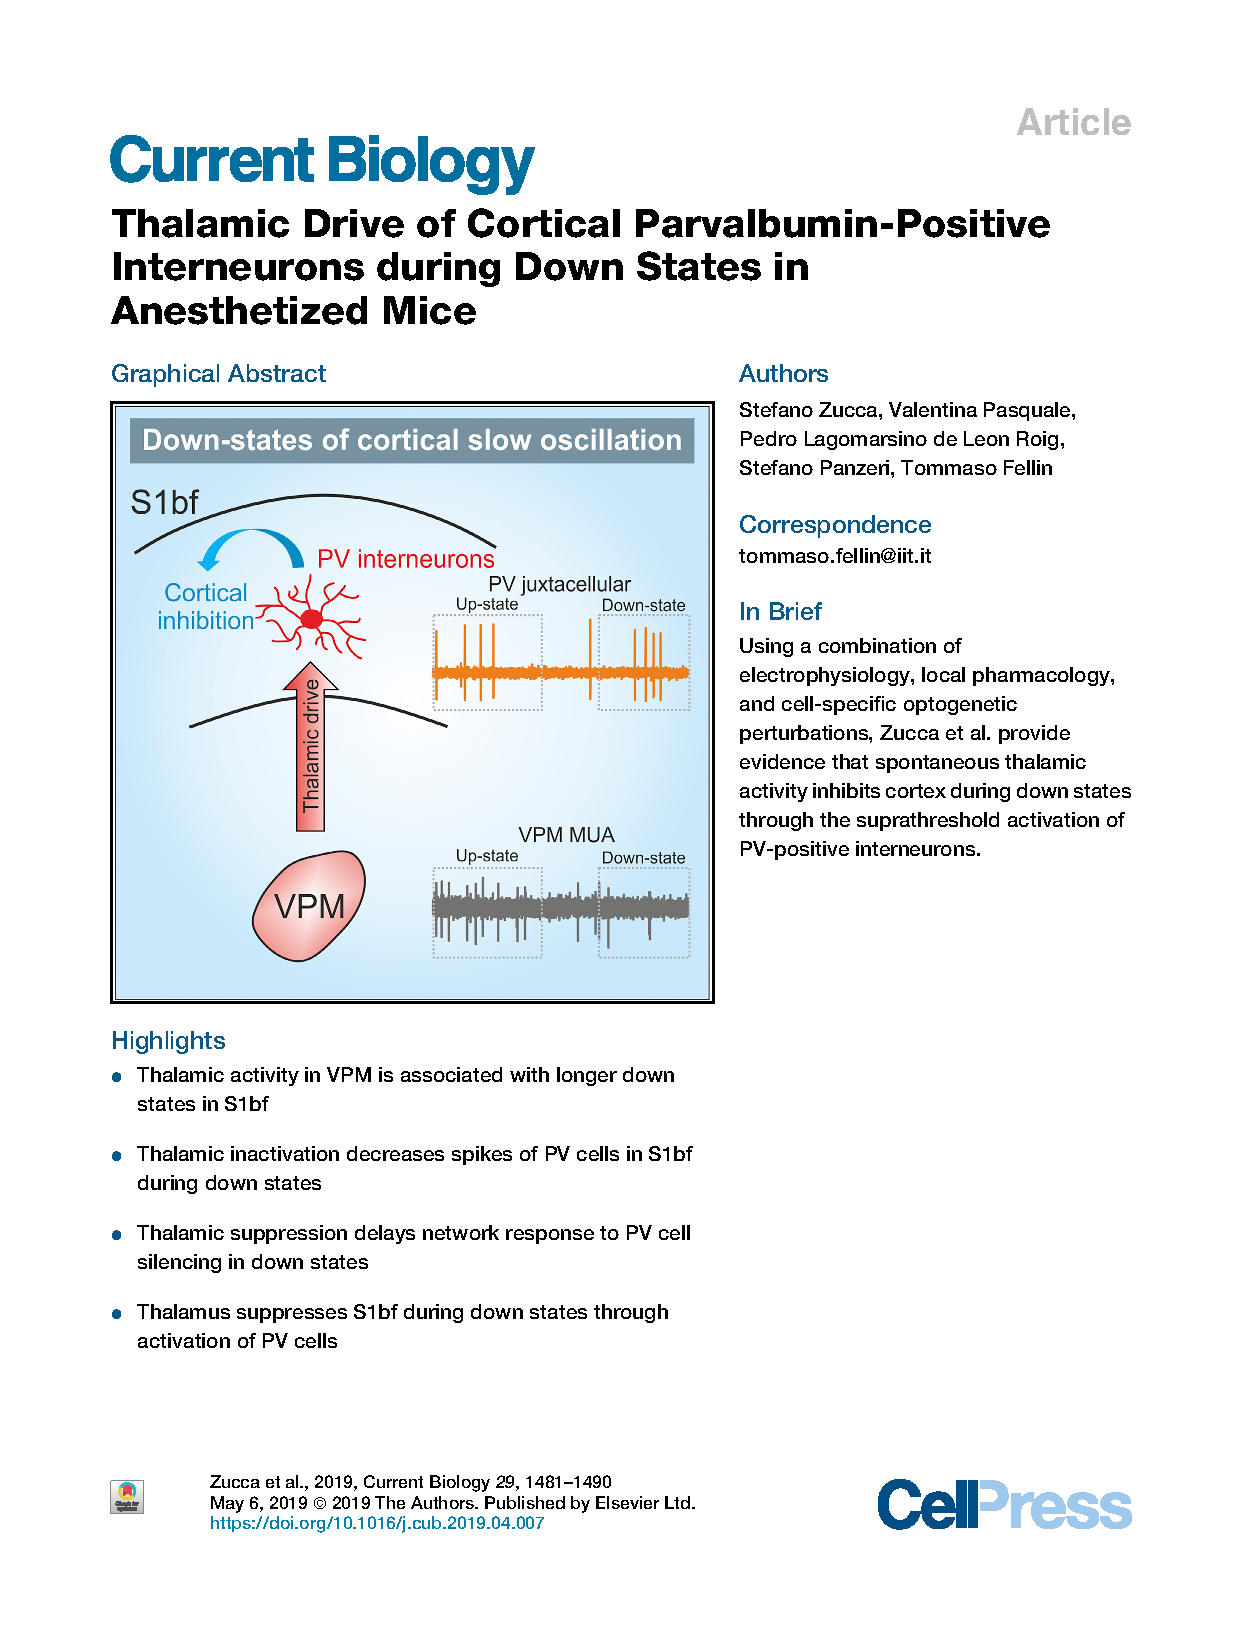
\includepdf[pages=-,pagecommand={\thispagestyle{plain}}]{pasquale_paper.pdf}

% Appendix Template

\chapter{Appendix Title Here} % Main appendix title

\label{AppendixX} % Change X to a consecutive letter; for referencing this appendix elsewhere, use \ref{AppendixX}

Write your Appendix content here.
% Appendix Template

\chapter{Appendix Title Here} % Main appendix title

\label{AppendixX} % Change X to a consecutive letter; for referencing this appendix elsewhere, use \ref{AppendixX}

Write your Appendix content here.


%----------------------------------------------------------------------------------------
%	BIBLIOGRAPHY
%----------------------------------------------------------------------------------------

\printbibliography[heading=bibintoc]

%----------------------------------------------------------------------------------------

\end{document}
